\documentclass[11pt,a4paper,twoside]{article}
\synctex=1
% LaTeX-Umsetzung der "Richtlinien f�r Projekt- und Diplomarbeiten"
% der LFE Medieninformatik, LMU M�nchen. (Autor: Richard Atterer, 27.9.2006, 23.10.2007), Bug-Fixing Mark Kaczkowski (23.6.2008)

\usepackage[T1]{fontenc} % sonst geht \hyphenation nicht mit Umlauten
\usepackage[latin1]{inputenc} % man kann schreiben ����, statt "a"o"u"s
%\usepackage[utf8]{inputenc} % wie oben, aber UTF-8 als Encoding statt ISO-8859-1 (latin1)
\usepackage[ngerman,english]{babel} % deutsche Trennregeln, "Inhaltsverzeichnis" etc.
%\usepackage{ngerman} % Alternative zum Babel-Paket oben
\usepackage{mathptmx} % Times-Roman-Schrift (auch f�r mathematische Formeln)
%\usepackage{natbib} % Cross references
% Zum Setzen von URLs
\usepackage{listings} % For displaying js source code
\lstdefinelanguage{JavaScript} {
	morekeywords={
		break,const,continue,delete,do,while,export,for,in,function,
		if,else,import,in,instanceOf,label,let,new,return,switch,this,
		throw,try,catch,typeof,var,void,with,yield
	},
  sensitive=false,
	morecomment=[l]{//},
	morecomment=[s]{/*}{*/},
	morestring=[b]",
	morestring=[d]'
}
% Code example
%\begin{lstlisting}[language=JavaScript]
%// create some nodes
%var headline = document.createElement(�h1�);
%var text = document.createTextNode(�Dies ist eine �berschrift�);
%// "offline" node manipulation
%headline.appendChild(text);
%// adding node to DOM
%document.getElementsByTagName("body")[0].appendChild(headline);
%\end{lstlisting}


\usepackage{color}
\definecolor{darkred}{rgb}{.25,0,0}
\definecolor{darkgreen}{rgb}{0,0.2,0}
\definecolor{darkmagenta}{rgb}{.2,0,.2}
\definecolor{darkcyan}{rgb}{0,.15,.15}
\usepackage[plainpages=false,bookmarks=true,bookmarksopen=true,colorlinks=true,
  linkcolor=darkred,citecolor=darkgreen,filecolor=darkmagenta,
  menucolor=darkred,urlcolor=darkcyan]{hyperref}

% pdflatex: Bilder in den Formaten .jpeg, .png und .pdf
% latex: Bilder im .eps-Format
\usepackage{graphicx}

\usepackage{fancyhdr} % Positionierung der Seitenzahlen
\fancyhead[LE,RO,LO,RE]{}
\fancyfoot[CE,CO,RE,LO]{}
\fancyfoot[LE,RO]{\Roman{page}}
\renewcommand{\headrulewidth}{0pt}
\setlength{\headheight}{13.6pt} % behebt headheight Warning

% Korrektes Format f�r Nummerierung von Abbildungen (figure) und
% Tabellen (table): <Kapitelnummer>.<Abbildungsnummer>
\makeatletter
\@addtoreset{figure}{section}
\renewcommand{\thefigure}{\thesection.\arabic{figure}}
\@addtoreset{table}{section}
\renewcommand{\thetable}{\thesection.\arabic{table}}
\makeatother
\sloppy % Damit LaTeX nicht so viel �ber "overfull hbox" u.�. meckert

% R�nder
\addtolength{\topmargin}{-16mm}
\setlength{\oddsidemargin}{25mm}
\setlength{\evensidemargin}{35mm}
\addtolength{\oddsidemargin}{-1in}
\addtolength{\evensidemargin}{-1in}
\setlength{\textwidth}{15cm}
\addtolength{\textheight}{34mm}
%______________________________________________________________________

\begin{document}

\pagestyle{empty} % Vorerst keine Seitenzahlen
\pagenumbering{alph} % Unsichtbare alphabetische Nummerierung

\begin{center}
  \textsc{University of Munich}\\
  Department ``Institute for Informatics''\\
  Education and Research Units Media Informatics\\
  Prof.\ Dr.\ Heinrich Hu�mann


\vspace{5cm}
{\large\textbf{Master Thesis}}\vspace{.5cm}

{\LARGE Web-Based Creator for Activity Sculptures}\vspace{1cm}

{\large Walter Rempening-Diaz}\\\href{mailto:me@walterrempening.com}{me@walterrempening.com}

\end{center}
\vfill

\begin{tabular}{ll}
  Working Time: & 1. 12. 2014 to 1. 6. 2015\\
  Supervisor: & Simon Stusak\\
  Responsible Professor: & Prof. Dr. Andreas Butz
\end{tabular}
%______________________________________________________________________

\clearpage
\section*{Acknowledgements}

\clearpage
\section*{Zusammenfassung}
Die Sammlung pers�nlicher Aktivit�tsdaten wurde durch die zahlreiche Anzahl an
Anwendungen und Ger�te enorm vereinfacht. Diese Anwendungen und
Ger�tschaften, die haupts�chlich das Ziel haben, Nutzer zu einem aktiven
Lebensstil ermutigen, k�nnen in Smarphones, wo sie die Vielfalt an Sensoren
ausnutzen oder als tragbare Accessoires wie moderne Uhren oder Armb�nder gefunden
werden. Abgesehen davon, dass klassische Datenvisualisierungen Einblicke in den
Aktivit�tsdaten verschaffen k�nnen, ist es auch m�glich den Datensatz durch
physikalische Objekte, auch als Aktivit�tsskulpturen bekannt, zu visualisieren.
Es wurde bewiesen, dass Aktivit�tsskulpturen Nutzer positiv beeinflussen, da die
Nutzer sich f�r ihren aktiven Lebensstil belohnt f�hlen. Um den Prozess der
Visualisierung von Information in Skulpturen weiter zu forschen wurde ein
Web-Konfigurator f�r Aktivit�tsskulpturen entwickelt. Durch die Nutzung moderner
Web-Technologien erh�lt der Nutzer eine Platform die ihm es erlaubt seine Daten
unkompliziert zu exportieren und erm�glicht ihn die Gestaltung einer 3D
druckbaren Skulptur. F�r die Entwicklung des Konfigurators, wurden aktuelle
Konfiguratoren analysiert mit dem Ziel Best-Practices im Bereich des Interface-
und Interaktionsdesigns zu erkennen. Um den Nutzer eine breite Vielfalt an
m�glichen Anpassungen f�r die Skulptur, wurden 4 verschiedene
Skulptur-Prototypen entwickelt. Letztendlich wurden f�r die Validierung des
Prototyps eine online Demoversion ver�ffentlicht und eine Nutzerstudie
durchgef�hrt. Die Resonanz der Nutzer zeigte, dass unser Prototyp einfach zu
bedienen war und, dass die entstandene Skulptur �sthetisch und sinnvoll r�berkam. 

\selectlanguage{english}
\section*{Abstract}
The recollection of personal activity data has been greatly facilitated by the
increasing amount of applications and devices that encourage users to measure
their activity with the primary goal of health improvement. These
devices range from mobile applications taking advantage of smartphone sensors to
dedicated fitness trackers presented as modern watches and bracelets. Apart from the
analytical insights about the data obtained through classic data
visualizations, it is also possible to visualize the information through
physical objects also known as activity sculptures. It has been shown that
activity sculptures have a positive influence in users making them feel rewarded
for their active lifestyle. To further study the process of visualizing activity
information into sculptures an web-based activity sculpture creator was
developed. This tool takes advantage of modern web
technologies and offers a platform in which users can export their data and
allows them to experiment creating variations of an activity sculpture which can also
be exported for 3D printing. For the development of the configurator current
product customization platforms where analyzed for gathering best practices in
user interface and interaction design. In order for users to have a sculpture
with a high degree of variability for the data to be mapped on 4 
different sculpture prototypes were developed. For the validation of the
configurator an online version was released and a user study was performed.
User feedback showed that our prototype was easy to operate and that the
obtained sculptures were appealing and meaningful them.


\cleardoublepage
\section*{Task Definition}
Activity Sculptures are physical (3D printed) representations of personal
tracking data (e.g.\ step count) that dwell between the artistic and the abstract. 
For this master's thesis the student will develop a web configurator that will
allow to individually create said activity sculptures (a similar example can be
seen in
\href{https://www.shapeways.com/creator/statement_vase}{www.shapeways.com/creator/statement\_vase}).\newline
The focus of the thesis will be the development of interaction concepts and
their implementation in the configurator. The concepts will be examined and
improved in smaller iterative user studies. Another important aspect is a
seamless and easy import of external tracking data (e.g.\ export data from tracking apps). The result should be a stable working prototype that can be used
for follow-up works.

\paragraph{Possible research questions}
\begin{itemize}
  \item What interaction concepts are possible? What are their advantages and
    disadvantages?
  \item What degree of freedom is possible and meaningful while designing a visualization?
  \item What is a possible design space for said activity sculptures?
\end{itemize}
\paragraph{Tasks}
\begin{itemize}
  \item Research and related works (e.g.\ data visualization, configurators)
  \item Development of interaction concepts
  \item Concept implementation
  \item Planing and executing several small user studies
  \item Written thesis and presentation of work
\end{itemize}
\paragraph{Requirements}
\begin{itemize}
  \item Programming skills in web development and computer graphics
\end{itemize}
\vfill % Sorgt daf�r, dass das Folgende an das Seitenende rutscht

\noindent I confirm that I independently prepared the thesis and that I used only
the references and auxiliary means indicated in the thesis. 
\bigskip\noindent 
\\Munich, \today

\vspace{4ex}\noindent\makebox[7cm]{\dotfill}

%______________________________________________________________________

\cleardoublepage
\pagestyle{fancy}
\pagenumbering{roman} % R�mische Seitenzahlen
\setcounter{page}{1}
% Inhaltsverzeichnis erzeugen
\tableofcontents

%______________________________________________________________________

\cleardoublepage

% Arabische Seitenzahlen
\pagenumbering{arabic}
\setcounter{page}{1}
% Ge�ndertes Format f�r Seitenr�nder, arabische Seitenzahlen
\fancyhead[LE,RO]{\rightmark}
\fancyhead[LO,RE]{\leftmark}
\fancyfoot[LE,RO]{\thepage}

%______________________________________________________________________
% Include Kapitel
%______________________________________________________________________

\cleardoublepage 
\chapter{Introduction}
\label{ch:intro}

\section{Inspiration}

And so it begins
%\_____________________________________________________________________

\cleardoublepage
\chapter{Background \& Related Work}
\label{ch:related}
\section{Background \& Related Work}
\subsection{Interactive Product Visualization}
\subsubsection{Gates 3D Configurator}
\subsubsection{Makervis}
\subsubsection{Twikit}
\subsection{Activity Sculptures}
\subsubsection{Sweet Atoms}
\subsubsection{Nike FuelBand Fibers}
\subsection{Activity Data Sources}
\subsubsection{Fitness Tracker API}
\subsection{Summary}

%______________________________________________________________________

\cleardoublepage
 % -*- root: ../medieninformatik-arbeit.tex -*-
\documentclass[../medieninformatik-arbeit.tex]{subfiles}
\begin{document}
\label{ch:proto}
\section{Prototype Design}
This chapter presents the process of developing the designs for the activity sculpture and the web configurator. In the first section the requirements for the activity sculpture are presented and four different designs that attempt to fulfill the requirements are presented. Finally the validation process for the sculpture to be designed will be discussed. The second section is devoted to the design process of the customization system. This comprehends not only the user interface but also the user experience while operating the system. After a process where three different concepts were ideated, through the validation of the design the final prototype is chosen. 

\subsection{Activity Sculpture Design}
The activity sculpture and the configurator are strongly interconnected as depending on the design, the sculpture will influence the quantity of controls to be taken into consideration for the design of the configurator giving users greater or lesser freedom for manipulating the the sculpture. As we discussed in section \ref{sec:activitysculptures}, activity sculptures portray different attributes inherit from their physical nature. This why a different approach for designing physical data visualizations is needed. For this purpose the design taxonomy proposed by Vande Moere et al.\cite{vande2009analyzing} was used as a guide to better categorize the qualities of the developed designs. This taxonomy is has two dimensions which describe the design space of activity sculptures: \textit{representational fidelity} and \textit{narrative formulation}. 

\textbf{The representational fidelity} attempts to explain the decision made for the embodiment of the data in form. This includes the chosen metaphor for mapping the data to the object and the resulting metaphorical distance, this is the level of abstraction used to represent the data through the metaphor. In order to better explain the abstraction level Vande Moere's taxonomy uses concepts from semiotic studies. According to C.K. Ogden et al.\cite{ogden1946meaning} semiotic signs can be explained through their three major concepts: the signified, the signifier and the sense. The signified is an object that represents a physical thing or and idea. The signified is represented by the signifier who tries to bring the same experience an observer would have with the signified. The sense is the experience brought by the signified. Furthermore signs can be categorized into iconic, indexical and symbolic. Iconic representation occurs when the signifier resembles the signified, like a picture or a diagram. Activity sculptures are iconic when they resemble  the metaphor they are interpreting. Examples of this could be the heart-beat extruded graph sculpture in discussed in section \ref{sub:sweatatoms} or the MakerVis visualizations in \ref{fig:makervis-config}. An indexical sign has a sensory feature that correlates directly to the signified. The signifier points to the signified through an actual connection, like dark clouds point to a forthcoming rain or smoke points to fire. Activity sculptures can be classified as indexical when through the use of a property directly related to the data. An example of such a sculpture would be the SweatAtoms frog in section \ref{sub:sweatatoms} or the . The most complex kind of sing is the symbol, as it does not bear any resemblance to the signified. The relationship between the signified and the signifier has to be taught by convention in order to be understood. Activity sculptures making use of symbolic representation are the hardest to understand as the relationship to the data has to be learned as it is not apparently displayed. Example of symbolic sculptures would be the landscapes in the Mental Fabrications project discussed in section \ref{sub:mentalfabrications}. Through the definition of iconic, indexical and symbolic representation we can derive their metaphorical distance resulting in indexical having the closest distance, symbolic the furthest and iconic a medium distance\cite{swaminathan2014supporting}. 

\textbf{The narrative formulation} of activity sculptures is a product of the physical form and the affordance of the object which influences the user's ability to discover information through interaction and perception. This quality is strongly interconnected to the representational fidelity as the level of abstraction in which the data is presented will form the properties in which the sculpture communicates. As discussed in section \ref{sec:activitysculptures} the affordance of an object describes to the viewer the object's potential to perform an action. The level of abstraction of the sculpture will influence how inviting the object is to the viewer depending on the user's level of familiarity with the metaphor used. 

Computer aided design systems offer almost endless possibilities in the design of activity sculptures, allowing designers to create complex structure designs that with manual methods it would be almost impossible to conceive.  Even though this might be the case in the digital realm, translating the virtual object into a physical object may be still a challenge. An important aspect to be considered while developing activity sculptures is the manufacturability of the sculpture\cite{swaminathan2014supporting}. 3D printing machines still are challenged by certain types of structures depending on the technology that is being used to manufacture (granular vs extrusion methods). Therefore it is important to take into account how challenging the manufacturability of the sculpture will be.

The the aforementioned design considerations of activity sculptures the requirements for the activity sculpture were formulated as follows. 

\begin{itemize}
	\item The sculpture has to be aesthetically appealing to users
	\item Motivate users to self reflection
	\item Because of the wide range of activity data types obtained through the fitness tracker, the sculpture has to be able to visualize as many variables as possible
	\item In order to provide users a relatively high level of freedom while customizing the sculpture, the sculpture has to offer multiple configuration options
	\item The sculpture has to be extended to new interaction forms
	\item The sculpture has to be 3D printable by current 3D printing technologies
\end{itemize}

With the defined requirements the author formulated four designs exploring different possible approaches. Due to space and layout considerations, the sketches drawn for the prototypes will not be displayed in this chapter only fragments. Due to the large sizes of the sketches all prototype sketches were placed in their entirety in the appendix of this work. For the sculpture prototypes sketches please refer to section \ref{App:proto-sculptures}, for configurator prototypes sketches refer to section \ref{App:proto-config}.

\subsubsection{3D Graph}
The first prototype is based on a line chart but augmented to describe more data variables. The idea was inspired by multiple exposure images of Olympic athletes in the middle of their performance. The multi exposure technique allows photographers to take a snapshot of the athlete at a specific point in time. The resulting image shows a group of athletes in different positions completing a cycle of a movement (see figure \ref{fig:multiexposure}). The concept of presenting snapshots of the athlete's position over time is actually a parallel concept to standard charts and charts where the value of a variable is presented at a specific point in time. Only transferring the line-chart to a physical space would have been not appealing enough and very limited as it would have been only possible to visualize one variable over time. The first modification made in order to improve the aesthetic of the sculpture was to give the chart-line volume and a triangulated or low polygon count (lowpoly) aesthetic, two properties that can be explored thanks to physical space. With this modification the sculpture gained the ability to visualize one more variable. The first variable influences the hight changes in the Y axis of the chart-line over time and by adding the volume to the line we can change the radius of the line according to the value changes of the variable over time. 

\begin{figure}[ht]
\captionsetup{width=0.8\textwidth}
\begin{center}
  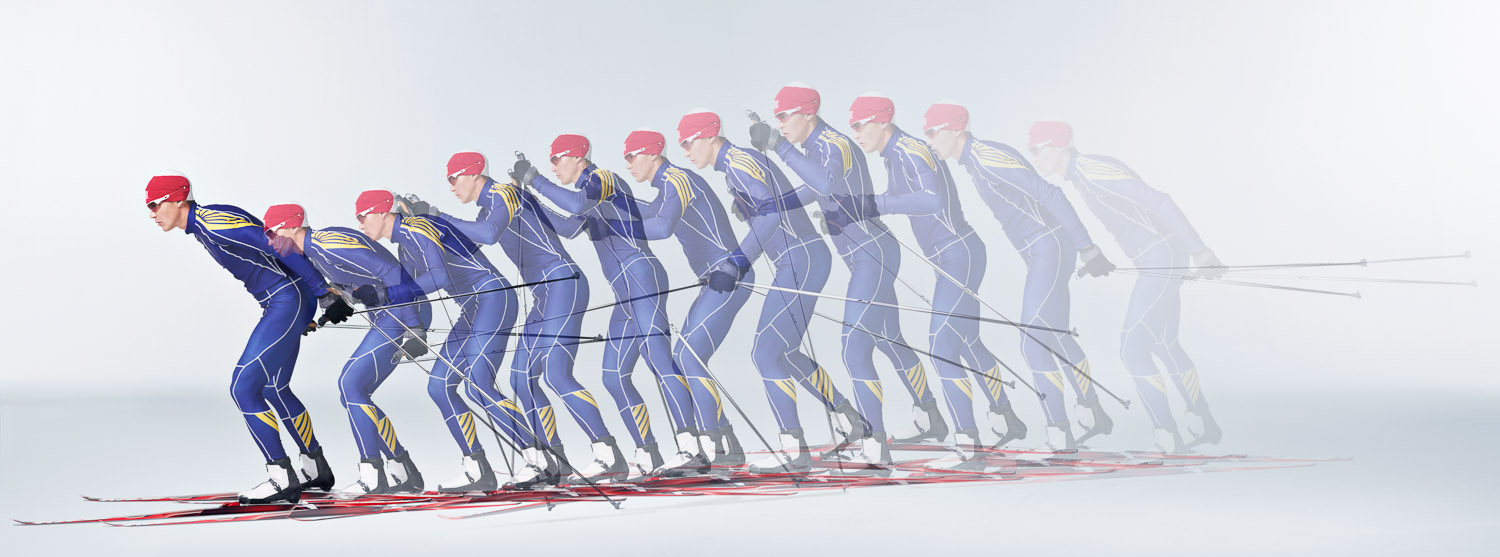
\includegraphics[width=0.8\textwidth]{Prototype/img/multiexposure}
  \caption{Athlete's movements captured in a multiple exposure image\cite{multiexposure}}
\label{fig:multiexposure}
\end{center}
\end{figure}

Up until this point the 3D graph would look as shown in figure \ref{fig:3DgraphDetail}. It visualizes up 2 variables over time. Even though the data is being visualized as an abstract triangulated body with hight and radius changes the sculpture could take advantage of the depth dimension not only to display volume but to steer the body also in this dimension. Through this realization, the 3D graph now can map 3 variables. To further enhance the aesthetic of the sculpture the concept of the athlete's snapshot in specific points of time was explored. For this a set of avatars performing different sports were developed. These avatars would intersect the graph body in specified intervals by the user. By adding different avatars performing a variety of sports users can chose the avatar that represents best the sport or activity the user did to generate the data. The sculpture could be expanded to support different decoration styles. For example apart from the triangulated look of the graph body, other visualization like a wire-frame option or a smoothed look could be offered. 
As shown in figure \ref{fig:3DgraphDetail}, the whole structure looks as if it would float in the air with the help of a support structure, which could be manufactured separately from transparent acrylic  so that they fade away centering the attention in the sculpture. This support structure would be inserted into a wooden or acrylic plate. The author explored the idea of engraving a summary of the data the sculpture represents. In this way users have both the abstract visualization and the actual data in the same place close enough to analyze. This might be useful while showing it to others, as it can help them better grasp how the sculpture was generated. By adding a plate to the sculpture we open a new set of configuration possibilities for users to edit in the configurator. 

The 3D graph embodies activity data through iconic and indexical representations. Indexical because as stated before, the concept emerged from an expanded line-chart an the graph body points to the path line-chart would have but abstracted and stylized and with the avatars in different positions point to movement in activity. The avatars are a strong icon of a human body in motion. The 3D graph shows a somewhat short metaphorical distance as the sculpture points strongly to the a line-chart metaphor used to embody the data. In the narrative formulation of the sculpture again the chart-graph resemblance and the plate tell the user this object is to be analyzed or at least admired as the plate does not allow grabbing the sculpture. Self reflection is highly encouraged as the metaphor motivates comparison of values over time. 

\begin{figure}[h]
\captionsetup{width=0.8\textwidth}
\begin{center}
  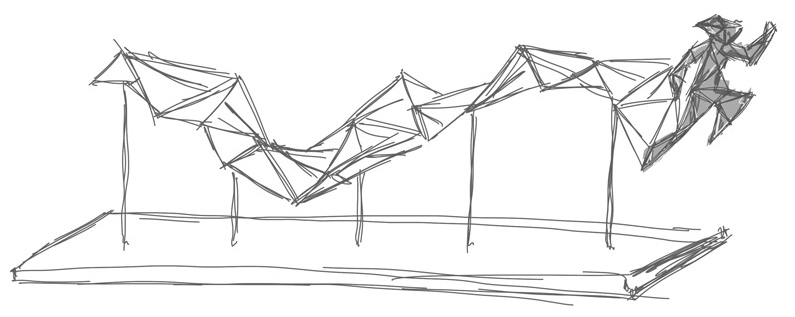
\includegraphics[width=0.8\textwidth]{Prototype/img/3DGraph_detail}
  \caption{3D Graph sketch}
\label{fig:3DgraphDetail}
\end{center}
\end{figure}

In summary, the 3D Graph prototype is a highly aesthetic activity sculpture that is also functional as the both the sculpture and the data could be analyzed in the same object. The sculpture can visualize data generated on a large time span. it has a rather low capability of mapping several variables because of the constraints of the line-chart metaphor. This could be improved by adding more graph bodies representing each 3 variables over time. The 3D graph offers a wide range of configuration options that would make it a rather interesting object to customize in the configurator. The manufacturability of the sculpture is attainable but also complicated as the sculpture, the plate and the supporting elements have to be fabricated not to mention the engravings on the plate. 

\subsubsection{Activity Landscape}
The activity landscape is an activity sculpture that embodies the data generated in a single day's activity by utilizing the data to generate a terrain (see figure \ref{fig:activitylandscape}. This concept of this sculpture came from the idea of generating a ground path from the GPS location points recollected while a user was jogging or riding his bike. After the workout other activity information like heart rate or elevation change would be mapped to the GPS locations. The user would then select in the configurator which variables he wants to map to different aspects of the terrain like and experiment with different variables for terrain elevation or map other variables to the radius of hills for instance. The activity landscape would also feature a plate for showcasing the sculpture. This plate as in the 3D Graph would feature engraved information about the work out like variables visualized, duration of the workout and calories burned. Because the terrain is based mostly on GPS information, the plate could also have an picture or engraving of a map where the workout was performed. As seen in section \ref{sub:sweatatoms} were some users stacked sculptures to form a bigger sculpture, several activity landscapes could be printed to form a bigger landscape. This could be used as a motivation to users to explore new parts of their city, it would be interesting to see how the landscape would look like after a year running or biking. This concept could also be applied to users who maybe travel constantly or like to ride their bikes in national parks around the world. After each travel they could bring the memories of their adventure in an activity landscape and put them together at their homes. 

\begin{figure}[h]
\centering
\begin{minipage}{.45\textwidth}
\centering
	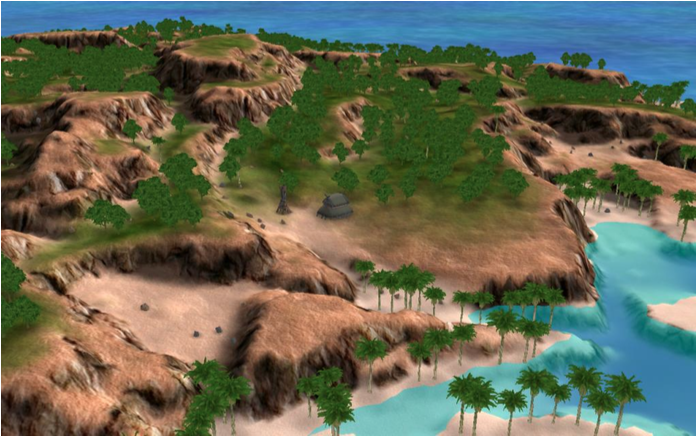
\includegraphics[width=\linewidth]{Prototype/img/terrain}
	\caption{Procedurally generated landscape \cite{olsen2004realtime}}
	\label{fig:proceduralterr}
\end{minipage}
\begin{minipage}{.45\textwidth}
\centering
  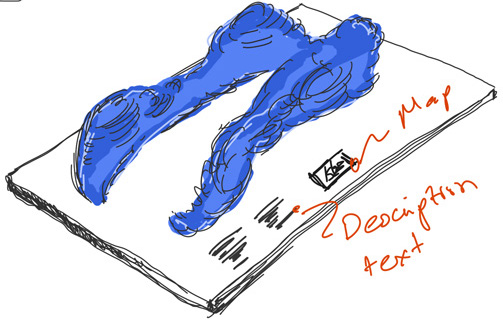
\includegraphics[width=0.88\linewidth]{Prototype/img/ActivityLandscape_detail}
  \caption{Activity Landscape sketch}
  \label{fig:activitylandscape}
\end{minipage}
\end{figure}

The inspiration of this idea was taken from the game development were with advances in processing power terrains for games are not being loaded from the assets library as 3D models bur rather generated in real time even with complex erosion simulations\cite{olsen2004realtime} (see figure \ref{fig:proceduralterr}). After looking at several generated terrains the concept of utilizing activity data to manipulate the generation of a terrain emerged. The configuration process would have been interesting to see as every time the user selected a different variable to manipulate the terrain, new sceneries would have emerged.

The activity landscape embodies the activity data through iconic representation as some of the terrain resembles some characteristics of the data like elevation and geographical position for example thus exhibiting a medium metaphorical distance. The level of affordance is low as it only invites the user to contemplate and self reflect. 

To summarize, the activity terrain provides an interesting approach to activity visualization and maybe also to procedural terrain generation in games. The level of customization in the configurator is high. It has to be clarified that the complexity of designing terrains was not studied in depth by the author, therefore it remains unknown how many variables are possible to visualize through the terrain. The added plate with the map can give users a stronger sense of belonging to their city. The idea of a personalized souvenir from adventure rides would be also interesting to explore. The sculpture does not exhibit any properties that could be proved difficult to manufacture. Same as the with the 3D Graph the plate could only make the fabrication process somewhat longer.  

\subsubsection{Activity Flora}
The activity flora is an activity sculpture that utilizes activity data as input parameters for the generation of a sculpture resembling a leaf. The concept for this prototype is to take the data generated in a single day or during a single workout and materialize it in a leaf like structure. In the sketch showed in figure \ref{fig:activityflora} activity data variables can be mapped to properties of the leaf. For example the size of the leaf could be affected by the traversed distance during that day, the contour shape could be mapped to elevation changes. The main branch in the middle of the leaf could be manipulated by the velocity changes, furthermore he characteristic branch structure inside the leaf could be influenced by the average heart-rate value (see figure \ref{fig:activityflora}). For the inner structure of the leave a generative system could be implemented to simulate better the leaf structure. In the configurator users could select which variable to map to each leaf generation parameter to generate a series of leafs. The customization possibilities could be further expanded with the addition of leaf tails and material options. To further explore the concept of grouping sculptures, a sketch with a stand that holds several leafs was drawn like a very stylized  flower pot. The leaf stand or pot would also be able to be customizable in the configurator.  

\begin{figure}[h]
\captionsetup{width=0.6\textwidth}
\begin{center}
  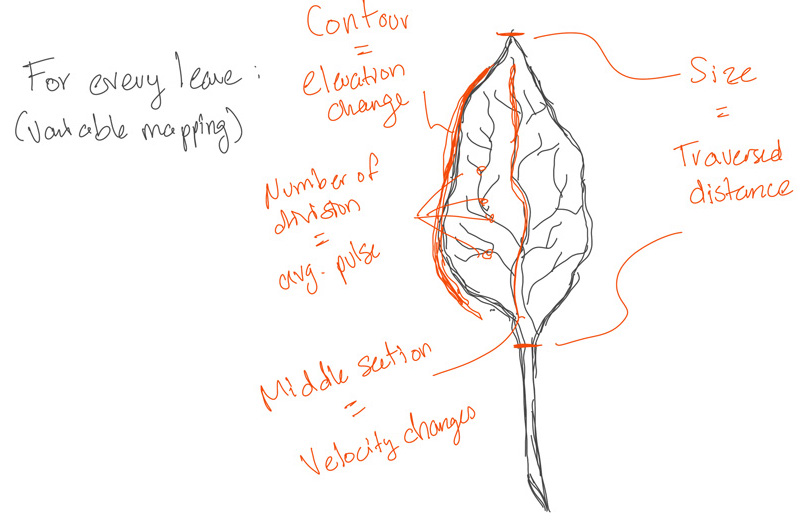
\includegraphics[width=0.6\textwidth]{Prototype/img/ActivityFlora_detail}
  \caption{Activity Flora sketch}
\label{fig:activityflora}
\end{center}
\end{figure}

The idea was inspired by the works of New York based generative design studio Nervous System\cite{nervousStudio} who since 2007 have been pioneering the design of generative objects for 3D printing. The majority of their designs is based in the simulation of natural structures or patterns through algorithms (see figure \ref{fig:nervous}. The concept of generating an object from activity data with an aesthetic inspired by nature was very appealing to the author. It would be interesting to see how users engage and perceive an object that was generated by their own activity but that also looks like something that lived, like a petrified leaf. Maybe in the future when 3D printing is also possible to do with biologic materials some kind of bacteria culture could be utilized to print the leaf alive for real. 

\begin{figure}[h]
\captionsetup{width=0.7\textwidth}
\begin{center}
  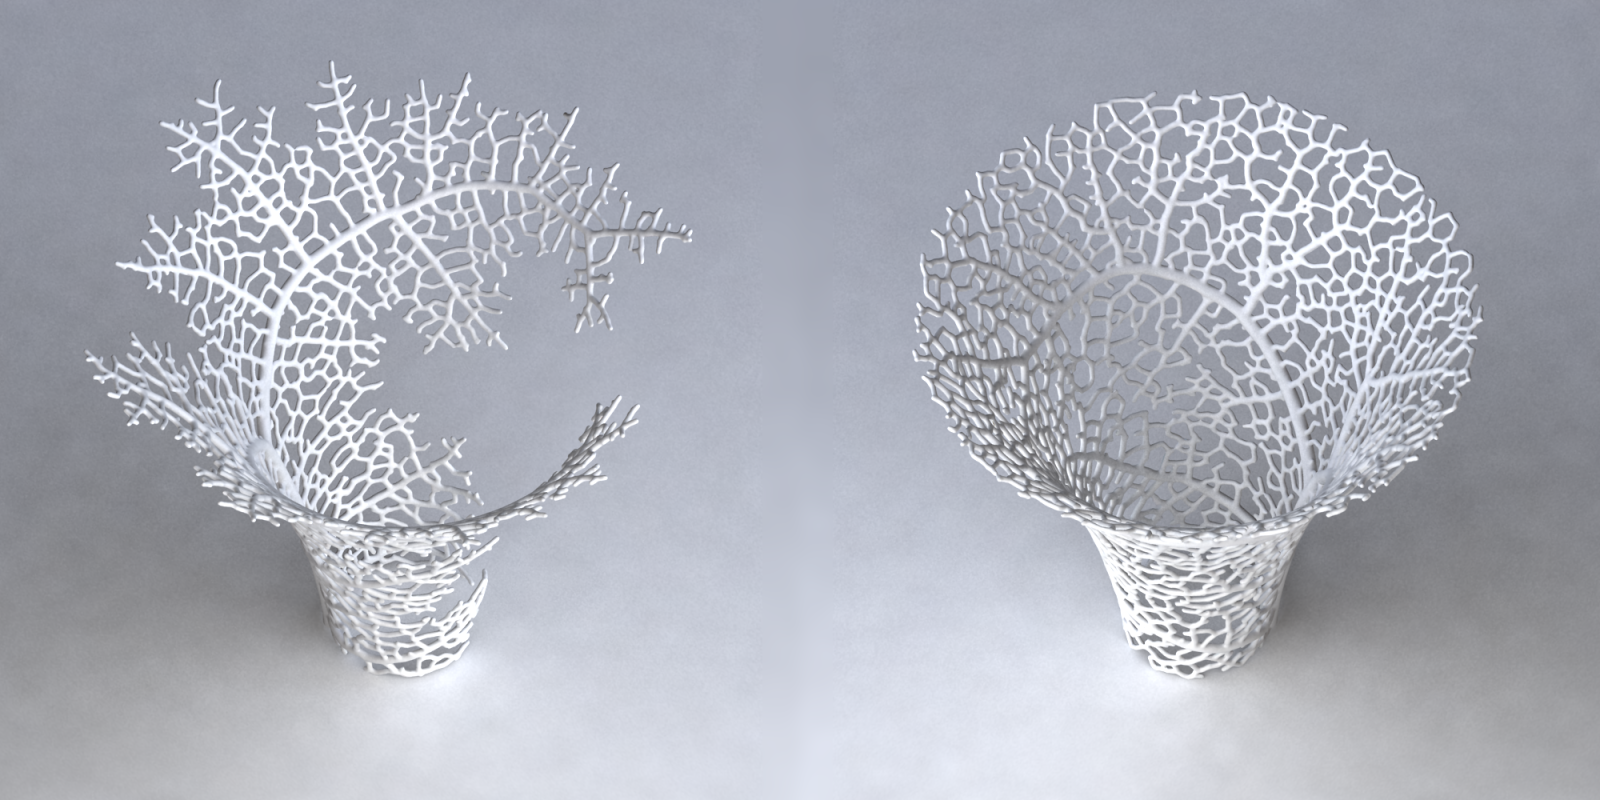
\includegraphics[width=0.7\textwidth]{Prototype/img/nervous}
  \caption{Sculptures made with generative algorithms based on hyphae growth as seen on leave and coral structures\cite{nervousHyphae}}
\label{fig:nervous}
\end{center}
\end{figure}

The activity flora embodies the data mostly iconic representation as the sculpture resembles a leaf but some information is abstracted completely because of the generative system resulting in a high medium metaphorical distance. The leaf prototype invites the user to contemplate the sculpture and due to the metaphor of the leaf self reflection will be harder for the viewer as the data is mapped not entirely to the sculpture but also to the system generating the leaf's structure.

To conclude this prototype, the activity leaf showcases a mixed approach to activity sculpture design, mapping some variables to physical properties of the leaf and using activity data as input for a generative system. The configuration possibilities are rather scarce and focus more on secondary elements of the sculpture like the stand or the leaf tail. The concept of metaphorically giving an object natural characteristics would be interesting to explore in the context of activity sculptures.

\subsubsection{Activity Vase}
The last developed prototype is the activity vase, a sculpture were the structure is conformed of a stacked radial chart with smoothly connected the axes. Every stacked radial chart represents a day's worth of activity. The user can choose in the configurator how many variables he wants to add to the vase by populating the radial chart. The height of the vase would be then configured by choosing the time span to be visualized which translates in the number of stacked radial charts (see figure \ref{fig:activityvase}. In this way the we can offer the user different outputs from one sculpture. Users could gain different usages of the sculpture depending on the visualized time span. For short time spans the sculpture could be expanded or adapted to be used as earrings or as a key-chain, longer time spans could be then used to make a pen holder or even a mug. Users could print each day the visualized data and maybe stacked them in a pole. As the sculpture better visualizes larger time spans from at least a day to weeks or months a sculpture representing two months in a year could be visualized, for example at the beginning and at the end of an intense workout plan an inner solid sculpture would represent the first month and an outer sculpture enclosing the first would represent the last month as it is expected that the activity performed will contain higher values in some variables, as the user reaches longer distances in their trainings for example. The sculpture could be further customized in the configurator through 3D printing material options and maybe even a simple plate were the labels of the variables are engraved. 

The concept of the activity vase was inspired by a 3D printed sculpture that maps two or more facial profiles to the sides of a vase and then unites them through extrusion. The final product is called Fhaz (see figure \ref{fig:fhaz}), which is basically an expansion of Rubin's vase\cite{rubin1921visuell} to visualize more than to profiles in a 3D printed object. In order to transfer the concept of Rubin's vase to an activity sculpture the idea of utilizing a stacked radial chart proved to be a suitable solution.

Using Vande Moere's taxonomy, the activity vase embodies the activity data through a symbolic representation as the visualization has no resemblance to the metaphor. As the abstraction of the represented data in the sculpture is high the metaphorical distance is also high. The activity vase offers viewers the freedom to explore the sculpture through touch and self-reflection because of the viewer's low familiarity with the object. The narrative has to be figured out through exploration and interaction with the object.

The activity vase is a very flexible sculpture in terms of data mapping. Through the radial chart metaphor the visualized amount of variables is only limited by the users decisions in the configurator. Due to its abstract representation the sculpture could be adapted to be used as everyday accessories and not only limited to standing in a shelf. The configurability of the sculpture is not very high but this could be addressed through the addition of different rendering styles like wire-frame to the configurator. The manufacturability of the sculpture is attainable as the solid structure of the vase does not challenge current fabrication methods. 


\begin{figure}[h]
\centering
\begin{minipage}{.45\textwidth}
\centering
	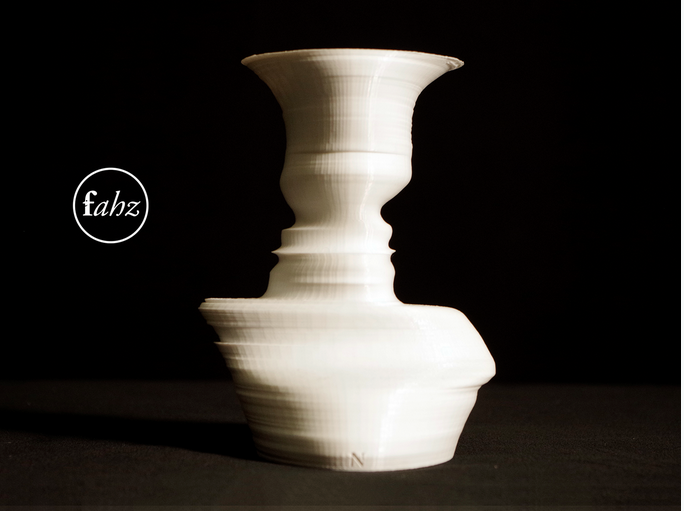
\includegraphics[width=\linewidth]{Prototype/img/fhaz}
	\caption{Fhaz: Procedurally generated vase based on facial profiles\cite{fahz}}
	\label{fig:fhaz}
\end{minipage}
\begin{minipage}{.45\textwidth}
\centering
  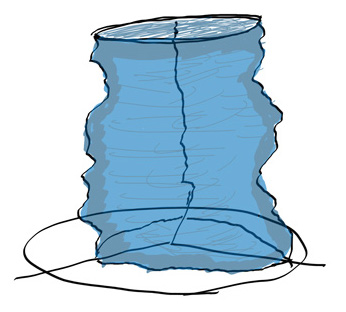
\includegraphics[width=0.75\linewidth]{Prototype/img/ActivityVase_detail}
  \caption{Activity Vase sketch}
  \label{fig:activityvase}
\end{minipage}
\end{figure}

\subsubsection{Prototype Validation}
After an extensive development process it was time to decide what prototype would be chosen to implement in for the web configurator. The decision was made by the author and the tutor through an iterative evaluation process. During the design process the prototypes were analyzed and discussed in order to discuss possible challenges or interesting concepts. Table \ref{tab:comparison} offers an overview of how each prototype compares to each other. For the analysis Vande Moere's taxonomy, the estimated complexity of the implementation of the sculpture and the customization capacity of the sculpture were considered. Estimating the implementation of the sculpture was vital, as the time of developing for the configurator and the sculpture were limited. The customization possibilities offered by the sculpture were also important as it was important to offer users an appealing sculpture that can be customized to their liking and more configuration options mean more unique sculptures. 

With this considerations in mind the activity vase fitted best the criteria. It is a very dynamic sculpture that offers a high variable mapping capability due to the radial chart metaphor, making it possible to visualize a high number of variables in the same sculpture. Unlike all other sculptures that are limited to 4 variables. The implementation complexity was estimated as medium because it can be achieved through common geometry construction algorithms. In comparison both the activity terrain and the activity leaf would have demanded a great amount of research on terrain generation and natural structure simulation. An important factor for choosing the activity vase was that it does not rely on a specific property of the data to be generated. For example the activity landscape depends heavily on GPS data to be generated. After analyzing the fitness-tracker that were intended to be used in this work, none of them supported GPS data. Due to the high cost of fitness-tracker that supported GPS and to the complexity of using a smartphone to address this issue, the activity terrain was discarded. The abstract nature of the activity vase, even though not familiar to most users it provides a representation that can be expanded to use in wearables or other artifacts that appeal to both genders, reaching in this way a wider audience. And finally it offers also a reasonable customization capacity that can be later expanded if needed. 

The final implementation of the sculpture and the possible control features will be discussed in Chapter \ref{ch:configurator} in section \ref{sub:sculpturegeneration}. Following the design process of the configurator will be discussed.   

\begin{table}[h]
\centering
\begin{tabular}{*{6}{|p{2.1cm}}|}
 \hline
 Sculpture Name & Metaphor & Semiotic Representation & Variable Mapping Capacity & Estimated Implementation Complexity & Customization Capacity \\
 \hline
 3D Graph & Line Chary & Indexical 	/Avatar Iconic & 4 & Medium high & Medium high\\
 \hline
 Activity Landscape & Terrain & Iconic & min. 2 & High & High\\
 \hline
 Activity Flora & Leaf & Iconic & 4 & High & Low\\
 \hline
 Activity Vase & Vase/	Cylinder & Symbolic & Unlimited & Medium & Medium\\
 \hline
\end{tabular}
\caption{Activity Sculpture Prototype Comparison}
\label{tab:comparison}
\end{table}

\subsection{Configurator Design}
\cite{abbasi2012s}
\cite{Konstanzer20078609220}
\cite{rolland2012commerce}

\subsubsection{Ideation Process}


\begin{figure}[h]
\captionsetup{width=0.9\textwidth}
\begin{center}
  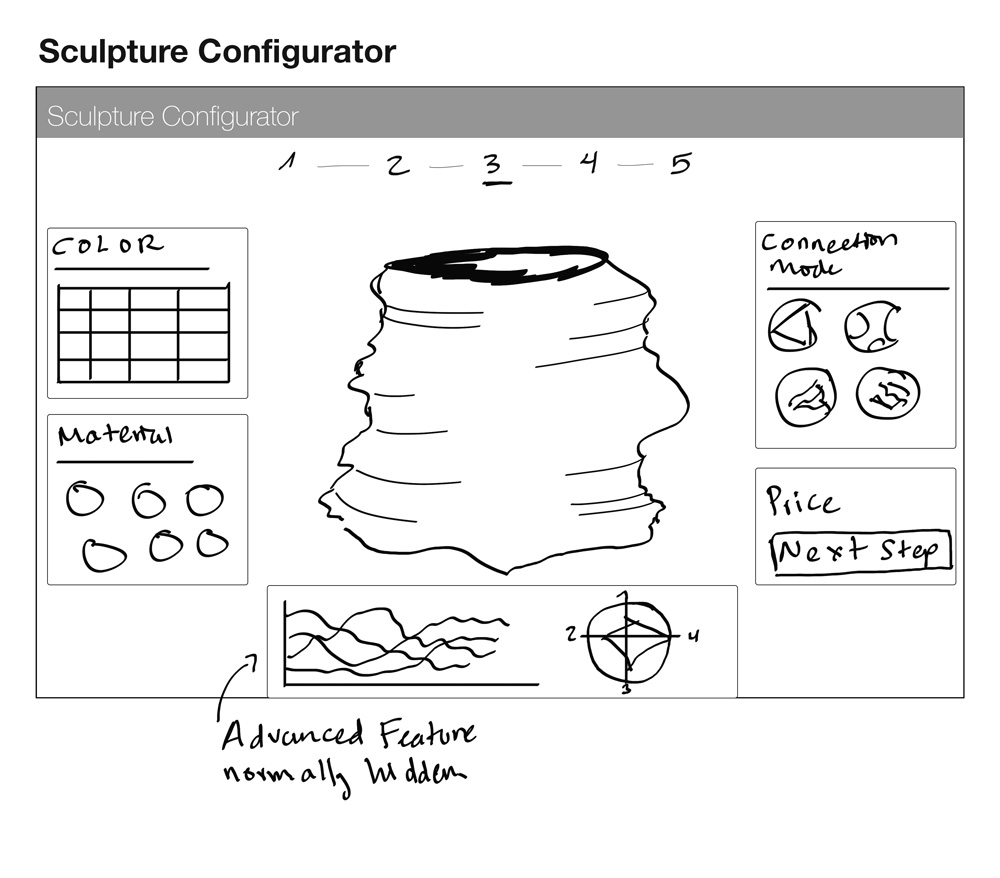
\includegraphics[width=0.6\textwidth]{Prototype/img/ui_proto1}
  \caption{Sketch of step based configurator prototype}
\label{fig:uiproto1}
\end{center}
\end{figure}

\begin{figure}[h]
\centering
\begin{minipage}{.45\textwidth}
\centering
  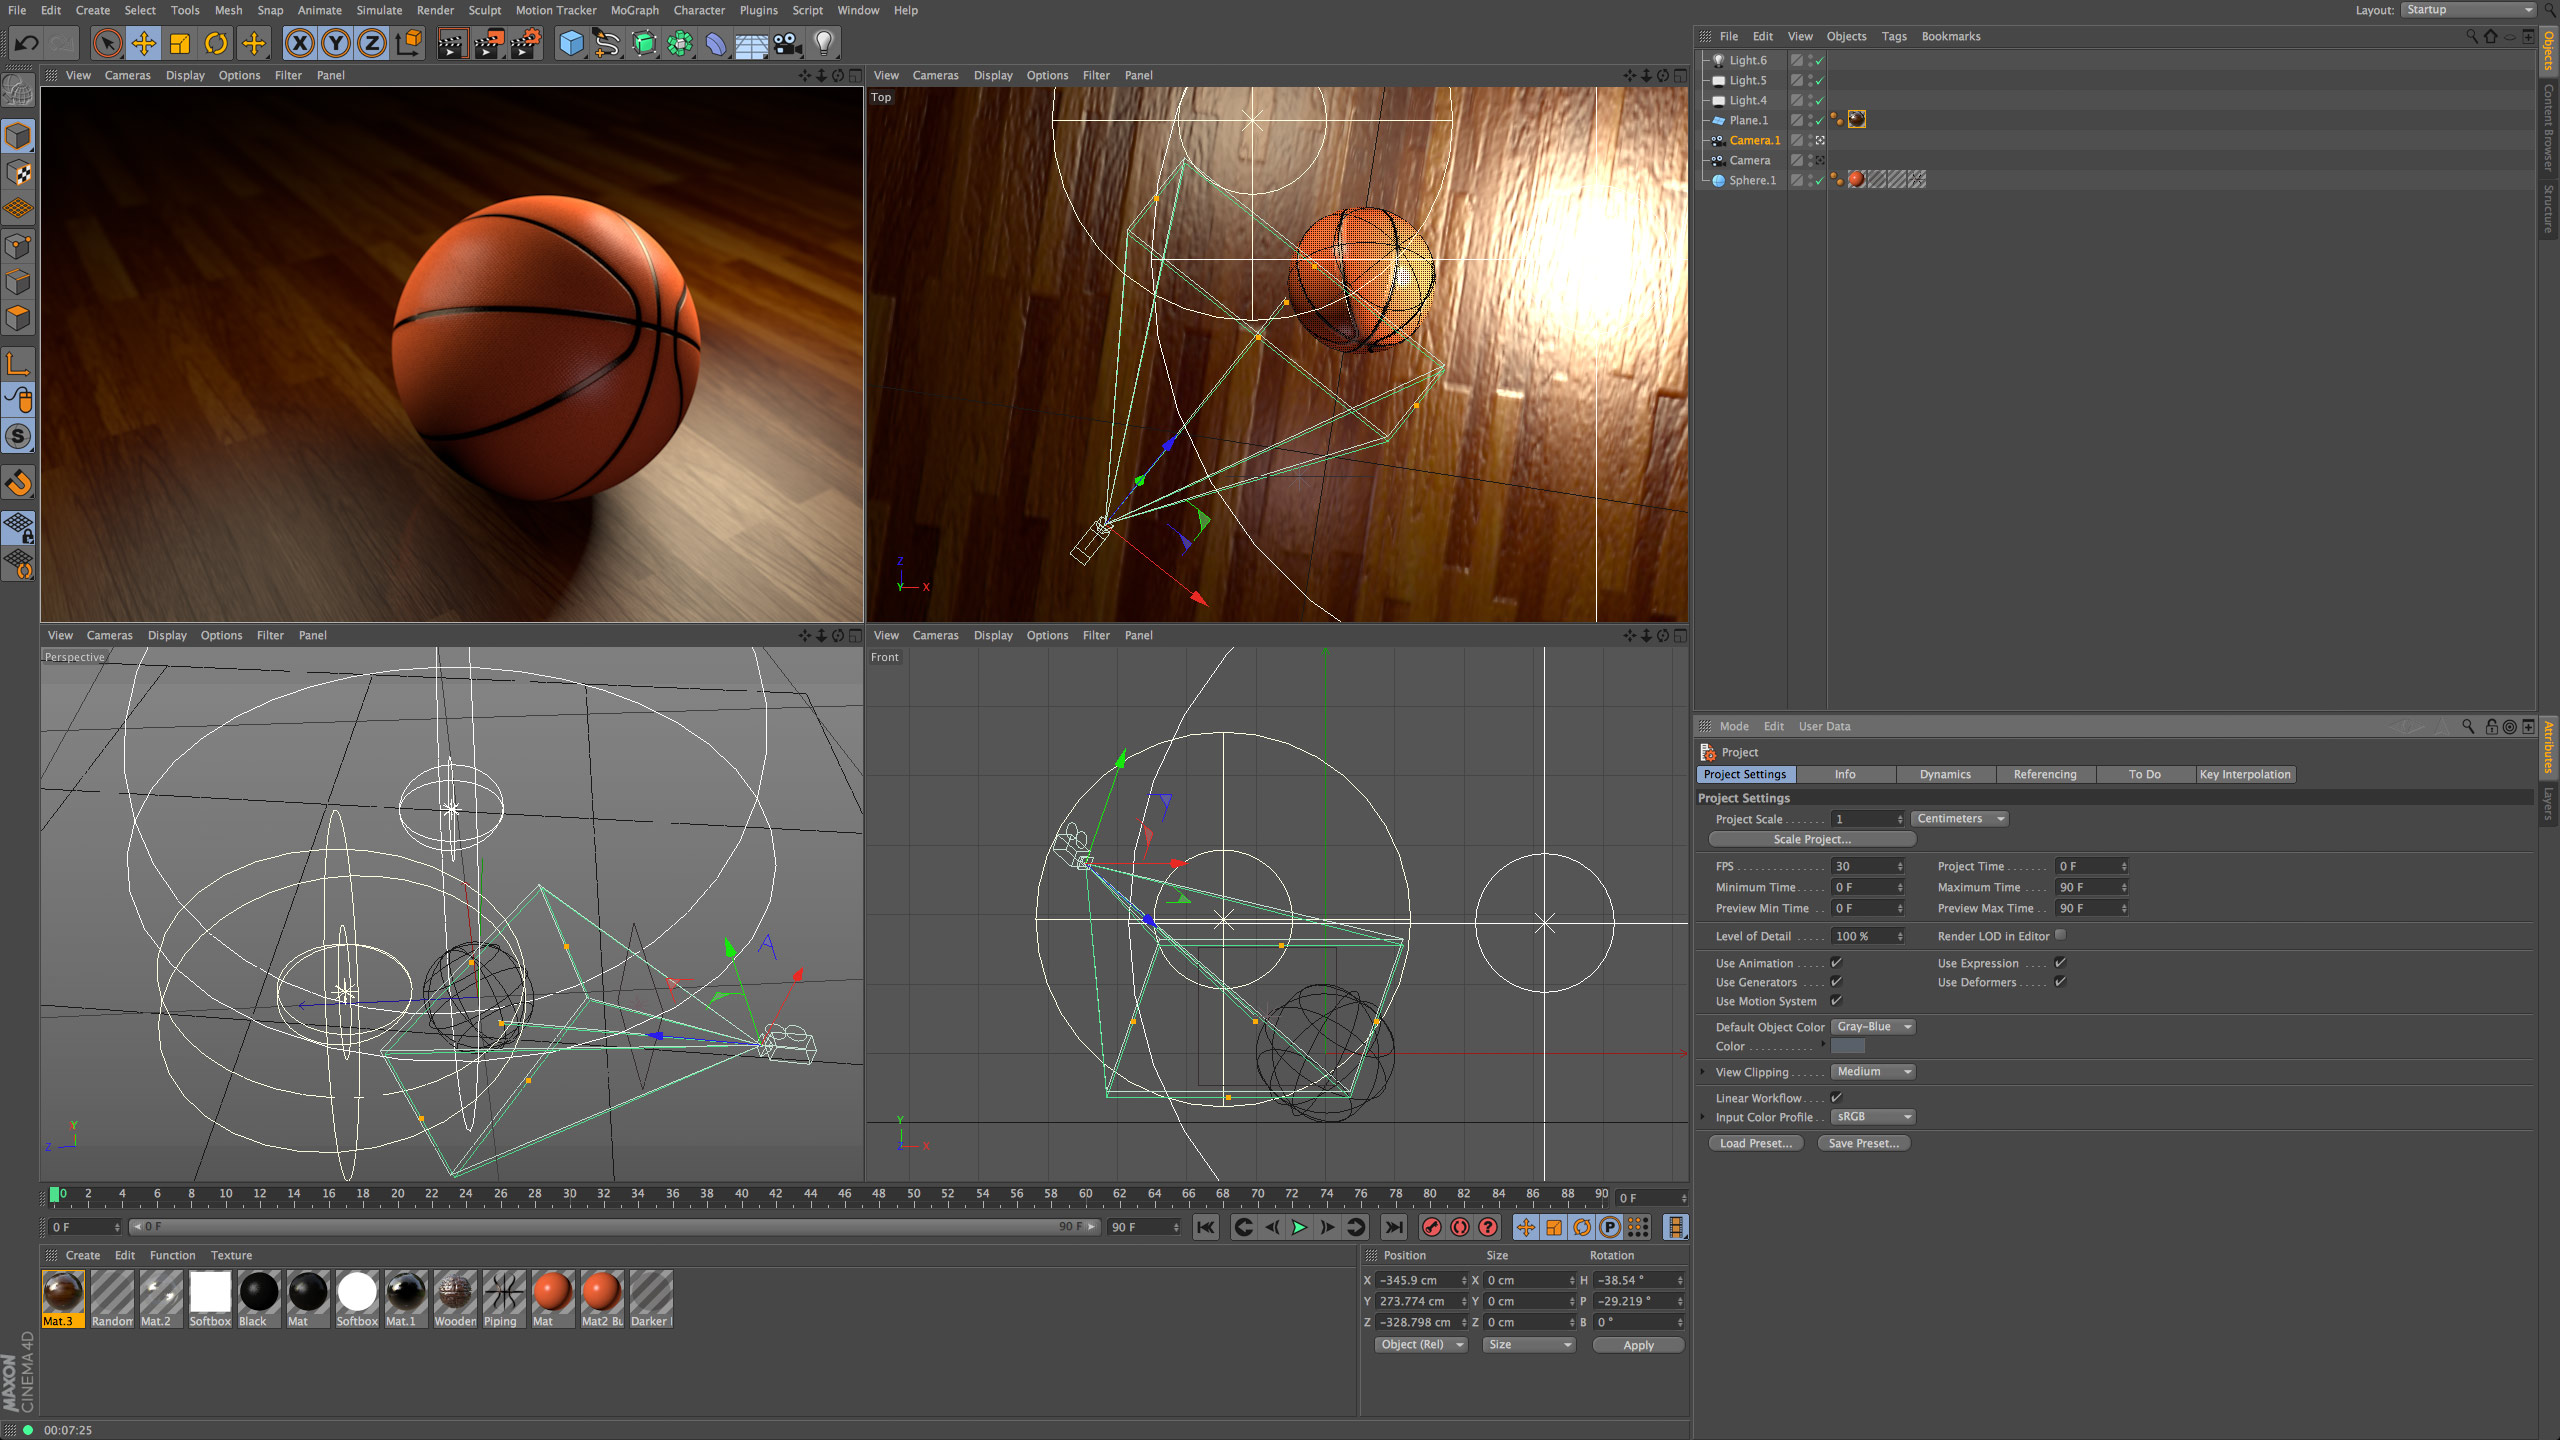
\includegraphics[width=\textwidth]{Prototype/img/cinema4d}
  \caption{3D modeling software Cinema 4D graphical user interface\cite{cinema4d}}
  \label{fig:cinema}
\end{minipage}
\begin{minipage}{.45\textwidth}
\centering
  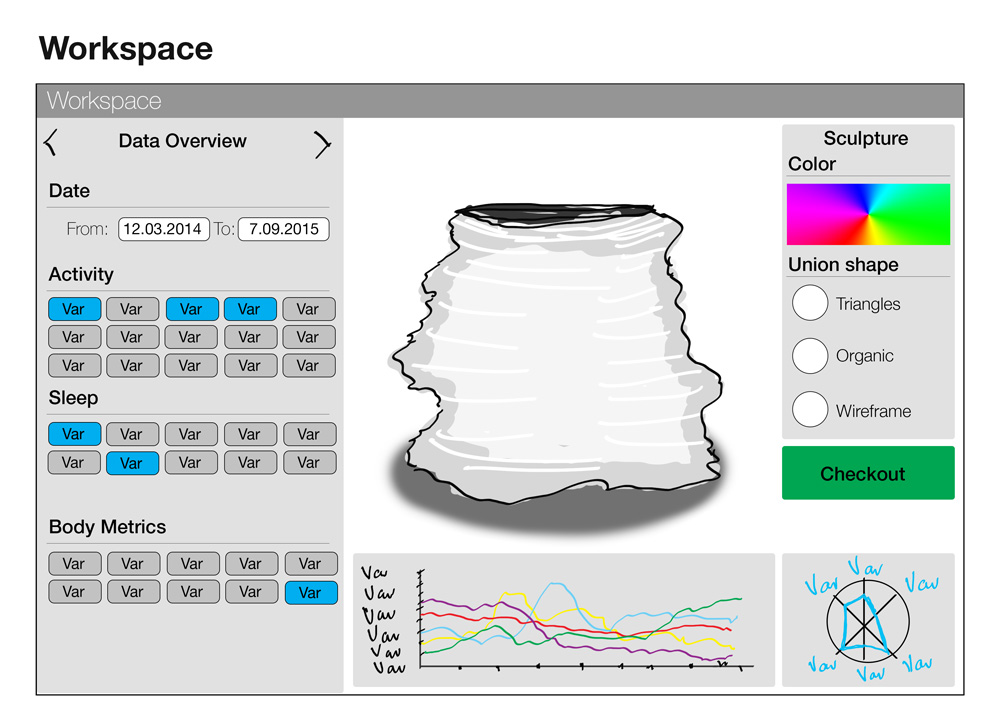
\includegraphics[width=\linewidth]{Prototype/img/ui_proto2}
  \caption{Sketch of 3D modeling software inspired configurator prototype}
  \label{fig:uiproto2}
\end{minipage}
\end{figure}

\begin{figure}[h]
\captionsetup{width=0.9\textwidth}
\begin{center}
  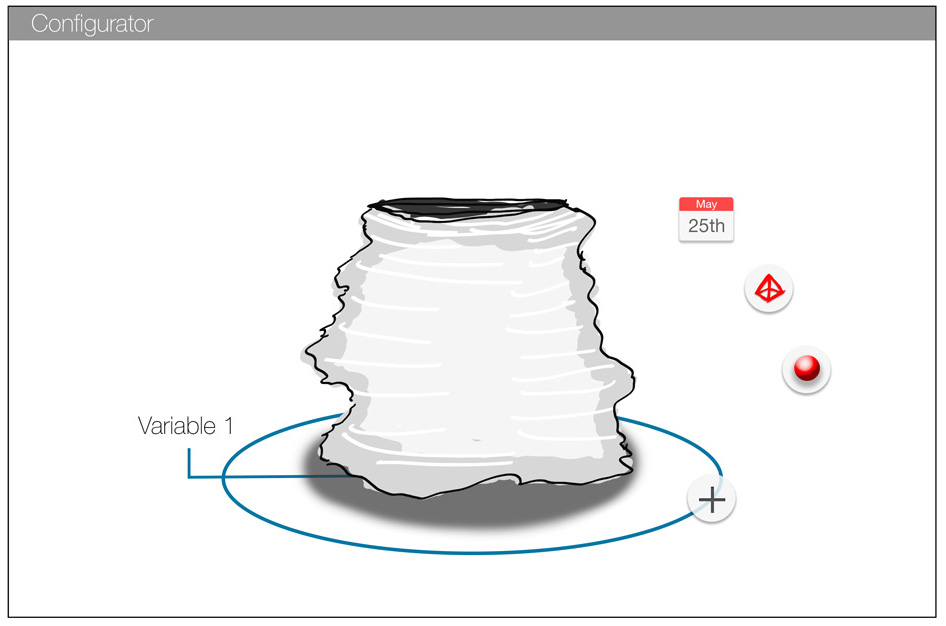
\includegraphics[width=0.6\textwidth]{Prototype/img/ui_proto3}
  \caption{Sketch of ``freestyle'' configurator prototype}
\label{fig:uiproto3}
\end{center}
\end{figure}

\subsubsection{Prototype Validation}

\end{document}
%______________________________________________________________________

\cleardoublepage
 % -*- root: ../medieninformatik-arbeit.tex -*-
\documentclass[../medieninformatik-arbeit.tex]{subfiles}
\begin{document}
\section{Implementation}
\label{ch:configurator}
The implementation of the activity sculpture configurator and the activity sculpture were undertaken in a period of around two months. The developed web configurator in this work makes use of cutting edge technologies for both web development and 3D visualization. This project is a demonstration of the capabilities of current web technologies that allow the developing of fully functional data visualization systems that offer integration with other web services for data interchange and support real time interactive 3D visualization.

This chapter will discuss all aspects of the technical implementation of the prototypes discussed in chapter \ref{ch:proto}. The technical requirements for the system will be discussed in the first section followed by an overview of the used technologies. Further on the modules conforming the system and their relationship will be explained in the architecture section. THe configurator section covers the implementation of the controls used by the user to manipulate the sculpture and the generation of the sculpture which are the main functionalities covered in the front end side of the application. The integration of the Whithings API and the manipulation performed on the received data are covered in the backend section of the chapter. Finally an overview of the challenges encountered while developing the system is presented. 

\subsection{Requirements}
Through the analysis of current works described in chapter \ref{ch:related},the requirements of the prototypes in chapter \ref{ch:proto} and in view of the forthcoming user study the functionality and technical requirements of the web-based activity sculpture creator were formulated as follows.

\begin{itemize}
	\item Implement the designed configurator workflow views
	\item Users have to be able to login with their personal Withings account
	\item Query user's data with the Withings API
	\item Store user's data and profile information in a data base
	\item Implement user interface control widgets like buttons, sliders and toggles for the customization area of the configurator
	\item Implement the designed activity sculpture geometry
	\item The visualization of the sculpture has to be rendered in real time  
	\item Changes made in the configurator have to be reflected in the sculpture instantly. avoid the use of update buttons 
	\item Users have to be able to navigate the sculpture in 3D space through rotation and zooming interactions
	\item STL file export support for 3D printing
	\item Support for current browsers
	\item Deployment of a fully working version in a web server for the general public. Anybody with a Withings account should be able to use it an visualize their data.
\end{itemize}


The required functionality is beyond what it would be needed for a basic working prototype. The developed configurator in this work is a fully functional system that fulfills every requirement specified in this section. The stated requirements involved the implementation of other functionality to ensure the requirement was fulfilled. For example the login functionality implies the implementation of an Oauth authentication solution(explained later in section \ref{sub:ApiIntegration}) in order to integrate with the Withings API. Also because the configurator is dealing with personal data the security of the system is important, as a basic approach to address this, the configurator implements session handling.

In the following section the used technologies to tackle the extensive list of requirements will be presented.  

\subsection{Technology}
The web configurator was developed with a modern stack of technologies that enable the use of the JavaScript language not only for frontend but also for the backend, the database and graphics programming. The MEAN stack is a collection of technologies that enables developers to write web applications in a single programming language. MEAN is the acronym for the technologies  conforming the stack: \textit{MongoDB}\cite{mongodb}, \textit{Express}\cite{express}, \textit{AngularJS}\cite{angular} and \textit{Node.js}\cite{joyent2015node}. The acronym was first used by Valeri Karpov, MongoDB engineer, in a blog post\cite{meanstack} where he discussed the benefits of using the same language across all technologies involved. Among the benefits Karpov states their team have experienced an increment in the performance of the developed software and also in the team's productivity. In short the MEAN stack's frameworks will be introduced. 

\textbf{MongoDB} is an ``open-source, document database designed for ease of development and scaling''\cite{mongodb}. Document based are conformed of collections (the equivalent of tables) which can contain several documents (rows) that  to any schema are in essence JSON Objects (JavaScript Object Notation). MongoDB does not enforce any schema to the stored data, making it a very flexible environment to work with. In MongoDB queries are performed in JavaScript providing a seamless integration of the JavaScript language, from querying the information to structuring it in JSON objects. The stored JSON objects are encoded to the BSON format which stands for Binary JSON to enhance efficiency and provide additional data types. Even though working with a schema-less database brings great flexibility, it is recommendable to bring some consistency to the MongoDB documents. For this purpose an object modeling library called \textit{mongoose}\cite{mongoose} has found broad adoption in the developer community. Mongoose provides functionality to easily model the application's data with type casting, custom query functions and other niceties. To illustrate how a mongoose schema looks like, listing \ref{list:mongoose-schema} shows an excerpt of the user schema designed for the configurator.

\begin{lstlisting}[style=htmlcssjs, caption={An excerpt of the user mongoose schema},label=list:mongoose-schema]
// load the mongoose module
var mongoose = require('mongoose');
var Schema = mongoose.Schema;

var userSchema = new Schema({
  profile: {
    name: String, //data type definition
    gender: Number,
    age: Number,
    location: String
  },
// more fields... 
  settings: {
    startDate: Date,
    endDate: Date,
    show: Boolean
  },
  sculptures: {type: Array, "default": []}
});
\end{lstlisting} 

\textbf{Node.js}\cite{joyent2015node} and \textbf{Express}\cite{express} are the frameworks used to develop the web server of the application. Node.js is backend JavaScript, based on the ``V8'' chrome JavaScript runtime providing an event-driven architecture and non-blocking i/o allowing for high performance real time applications. \textit{Node.js} is conformed of basic modules that provide network functionality but it requires the developer to build everything from the ground up. To address this issue the JavaScript library \textit{Express} was developed. Express provides a rich set of features like routing, middleware support and HTTP utilities that allow rapid development of network applications. Listing \ref{list:node-server} shows how a simple server is implemented with Node.js and Express.

\begin{lstlisting}[style=htmlcssjs, caption={Basic Node.js and Express server example},label=list:node-server]
var express = require('express');
var app = express();

app.get('/', function (req, res) {
  res.send('Hello World!');
});

var server = app.listen(3000, function () {
  var host = server.address().address;
  var port = server.address().port;
  console.log('Example app listening at http://%s:%s', host, port);
});
\end{lstlisting}

\textbf{AngularJS}\cite{angular} is the fronted framework in the MEAN stack. \textit{AngularJS} is an opens-source project developed by Google for the development of Single Page Applications (SPAs) where the whole content of a web page is rendered in a single web page and the content is either completely loaded at the beginning or its injected according to user interactions. AngularJS is based on a Model-View-Whatever design pattern (MVW) that allows developers to choose the design pattern that better accommodates their coding style. Whichever design pattern is chosen, AngularJS enforces developers to structure code into modules providing a strong organization in the code base. The functionality provided by AngularJS ranges from bidirectional data-binding, routing, form validation, server communication tools and directives that allow the creation of custom HTML syntax. With frameworks like AngularJS SPA allow to take much of the server workload to the frontend. Another feature of AngularJS is its extensibility. For the purposes of this work the \textit{Angular Material}\cite{angularmaterial} was utilized to implement user interface controls and theming. The \textit{Angular Material} module is also developed by Google and it provides a solid framework for developing user interfaces utilizing the ``Material design'' philosophies. 

In the following sections the utilization the benefits of developing with the MEAN stack with other technologies will be highlighted through examples of modules developed for the web configurator. 

\subsection{Architecture}


\begin{figure}[h]
\captionsetup{width=\textwidth}
\begin{center}
  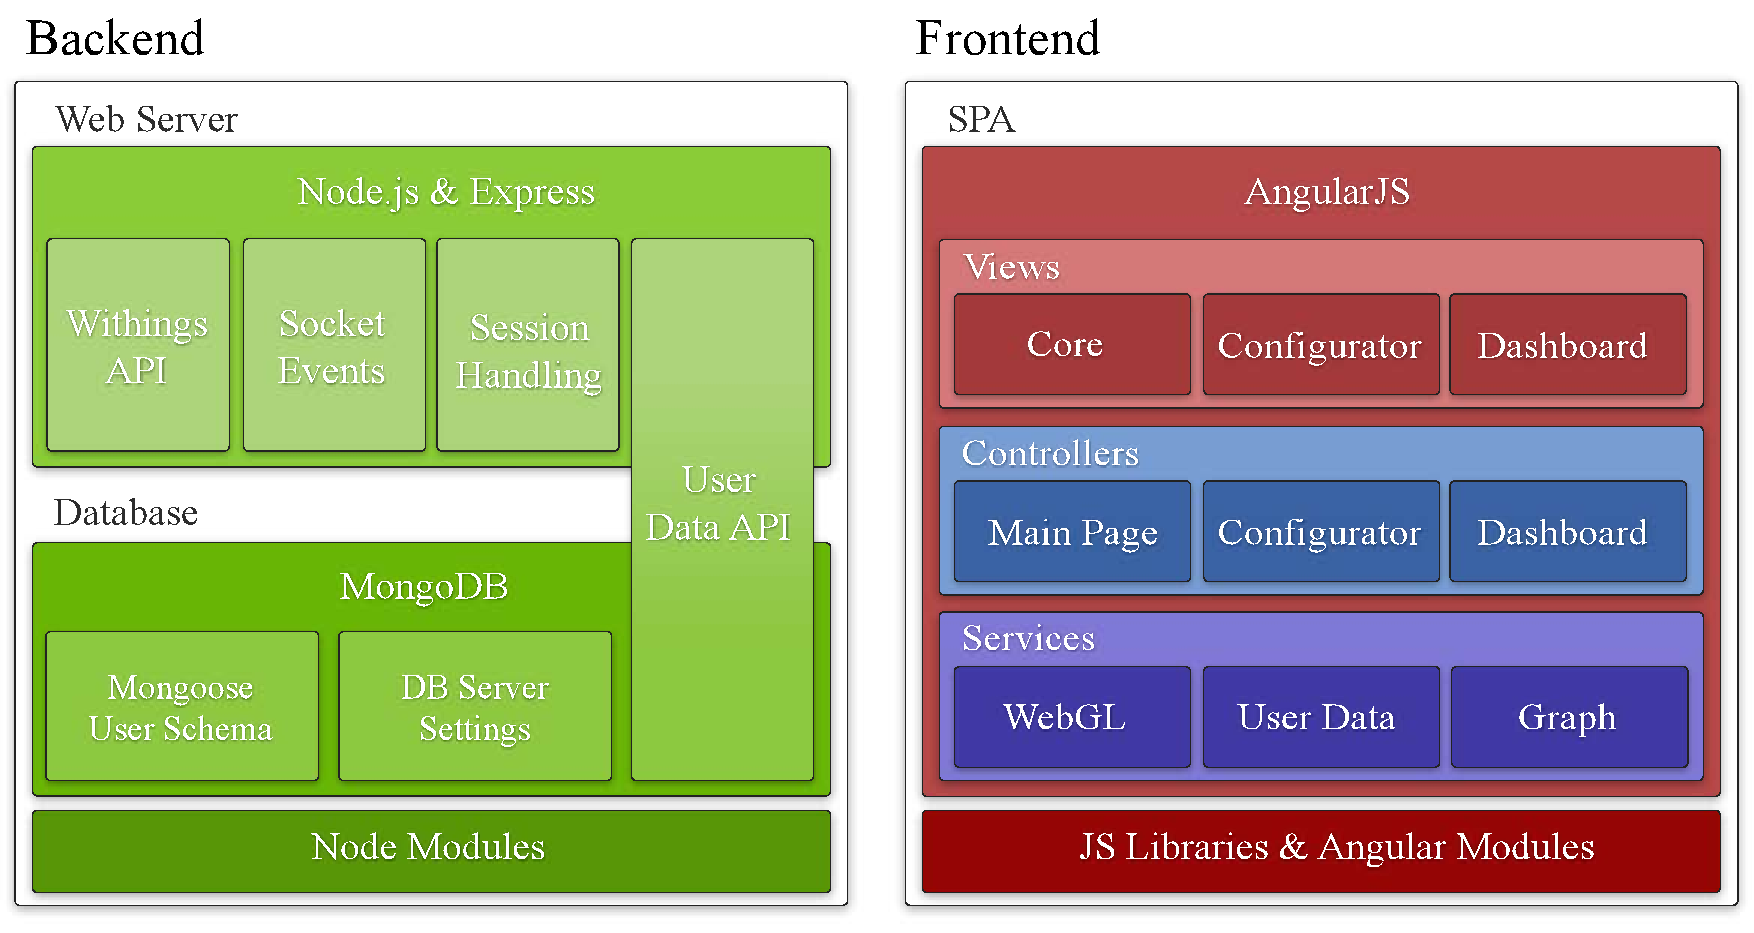
\includegraphics[width=\textwidth]{Configurator/img/Architecture}
  \caption{Activity Sculpture web configurator's architecture}
\label{fig:architecture}
\end{center}
\end{figure}

\begin{figure}[h]
\captionsetup{width=\textwidth}
\begin{center}
  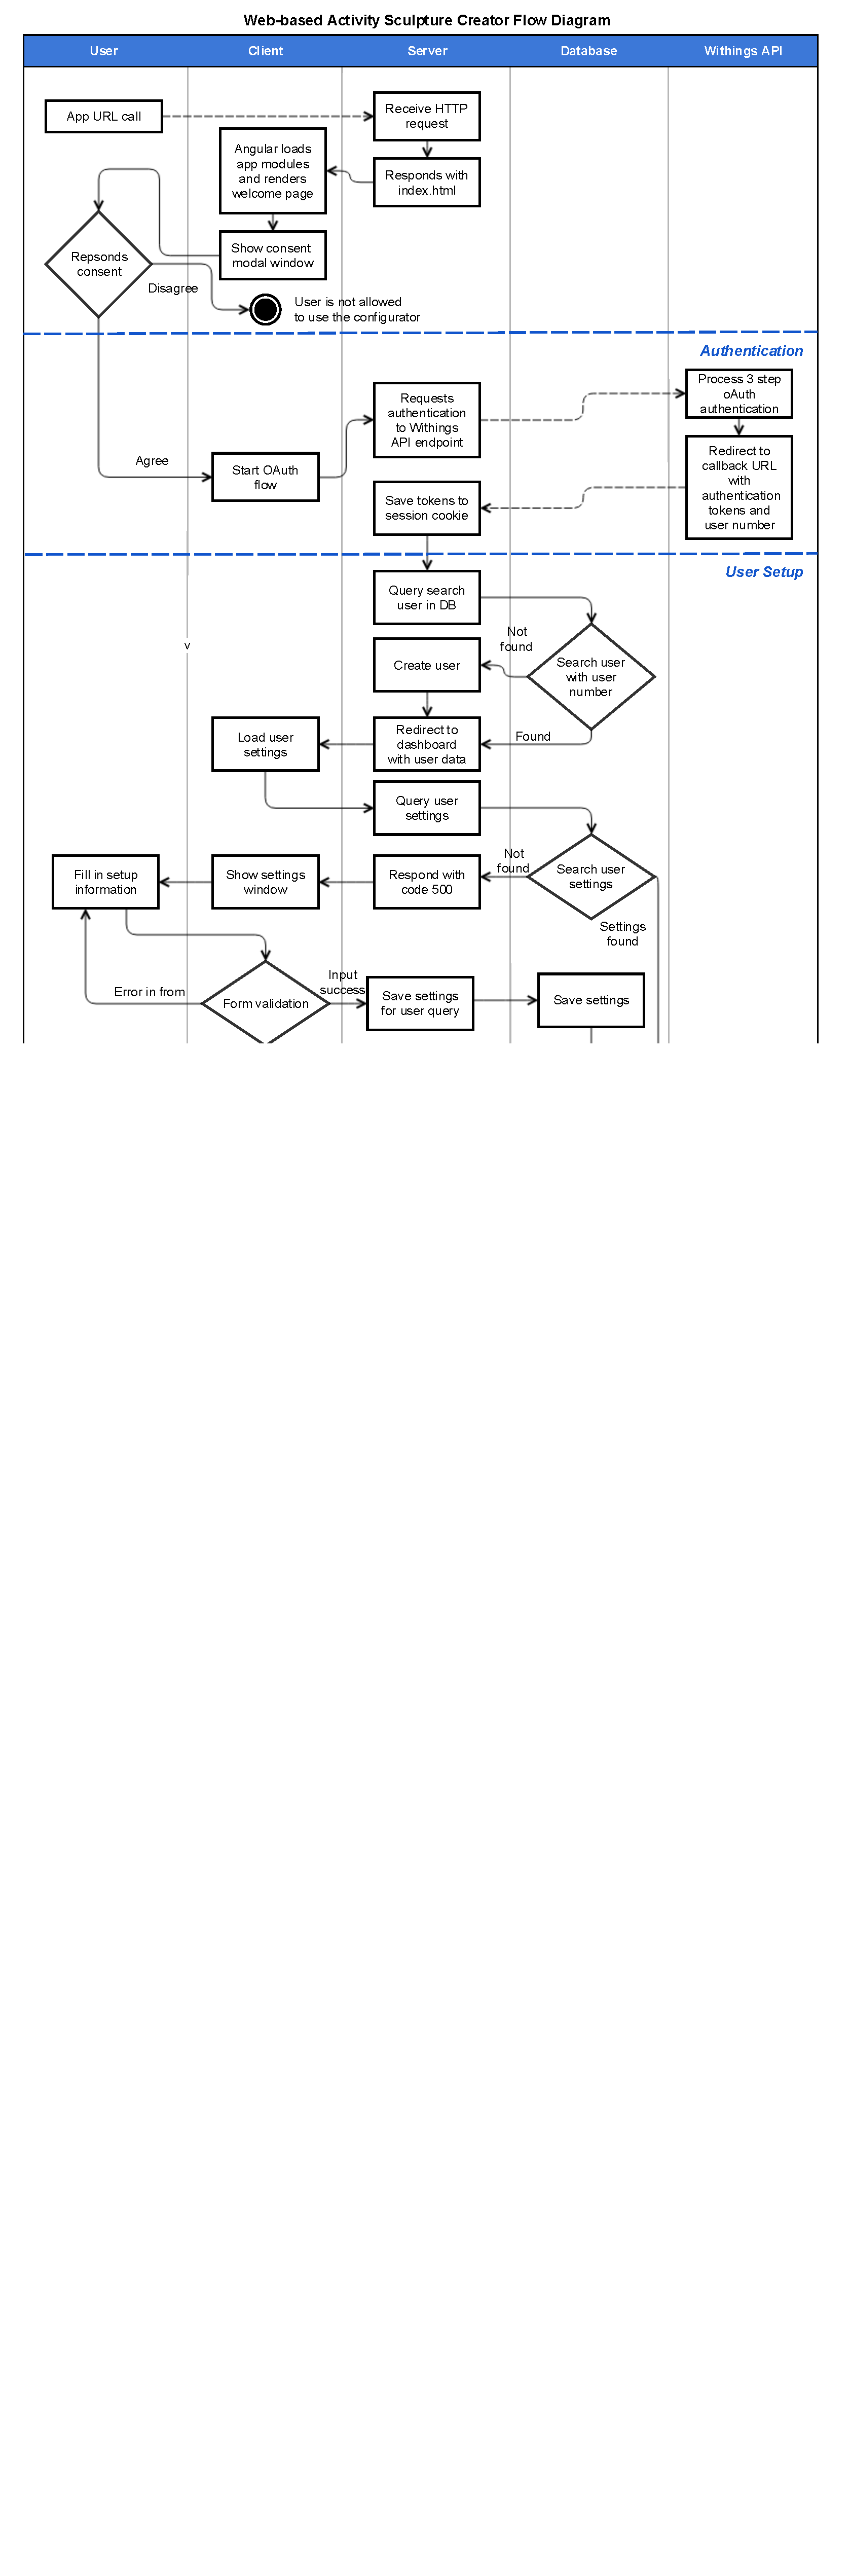
\includegraphics[width=0.9\textwidth]{Configurator/img/flowdiagram_1}
  \caption{Activity Sculpture web configurator's flow diagram part 1}
\label{fig:flowdiagram}
\end{center}
\end{figure}

\begin{figure}[h]
\captionsetup{width=\textwidth}
\begin{center}
  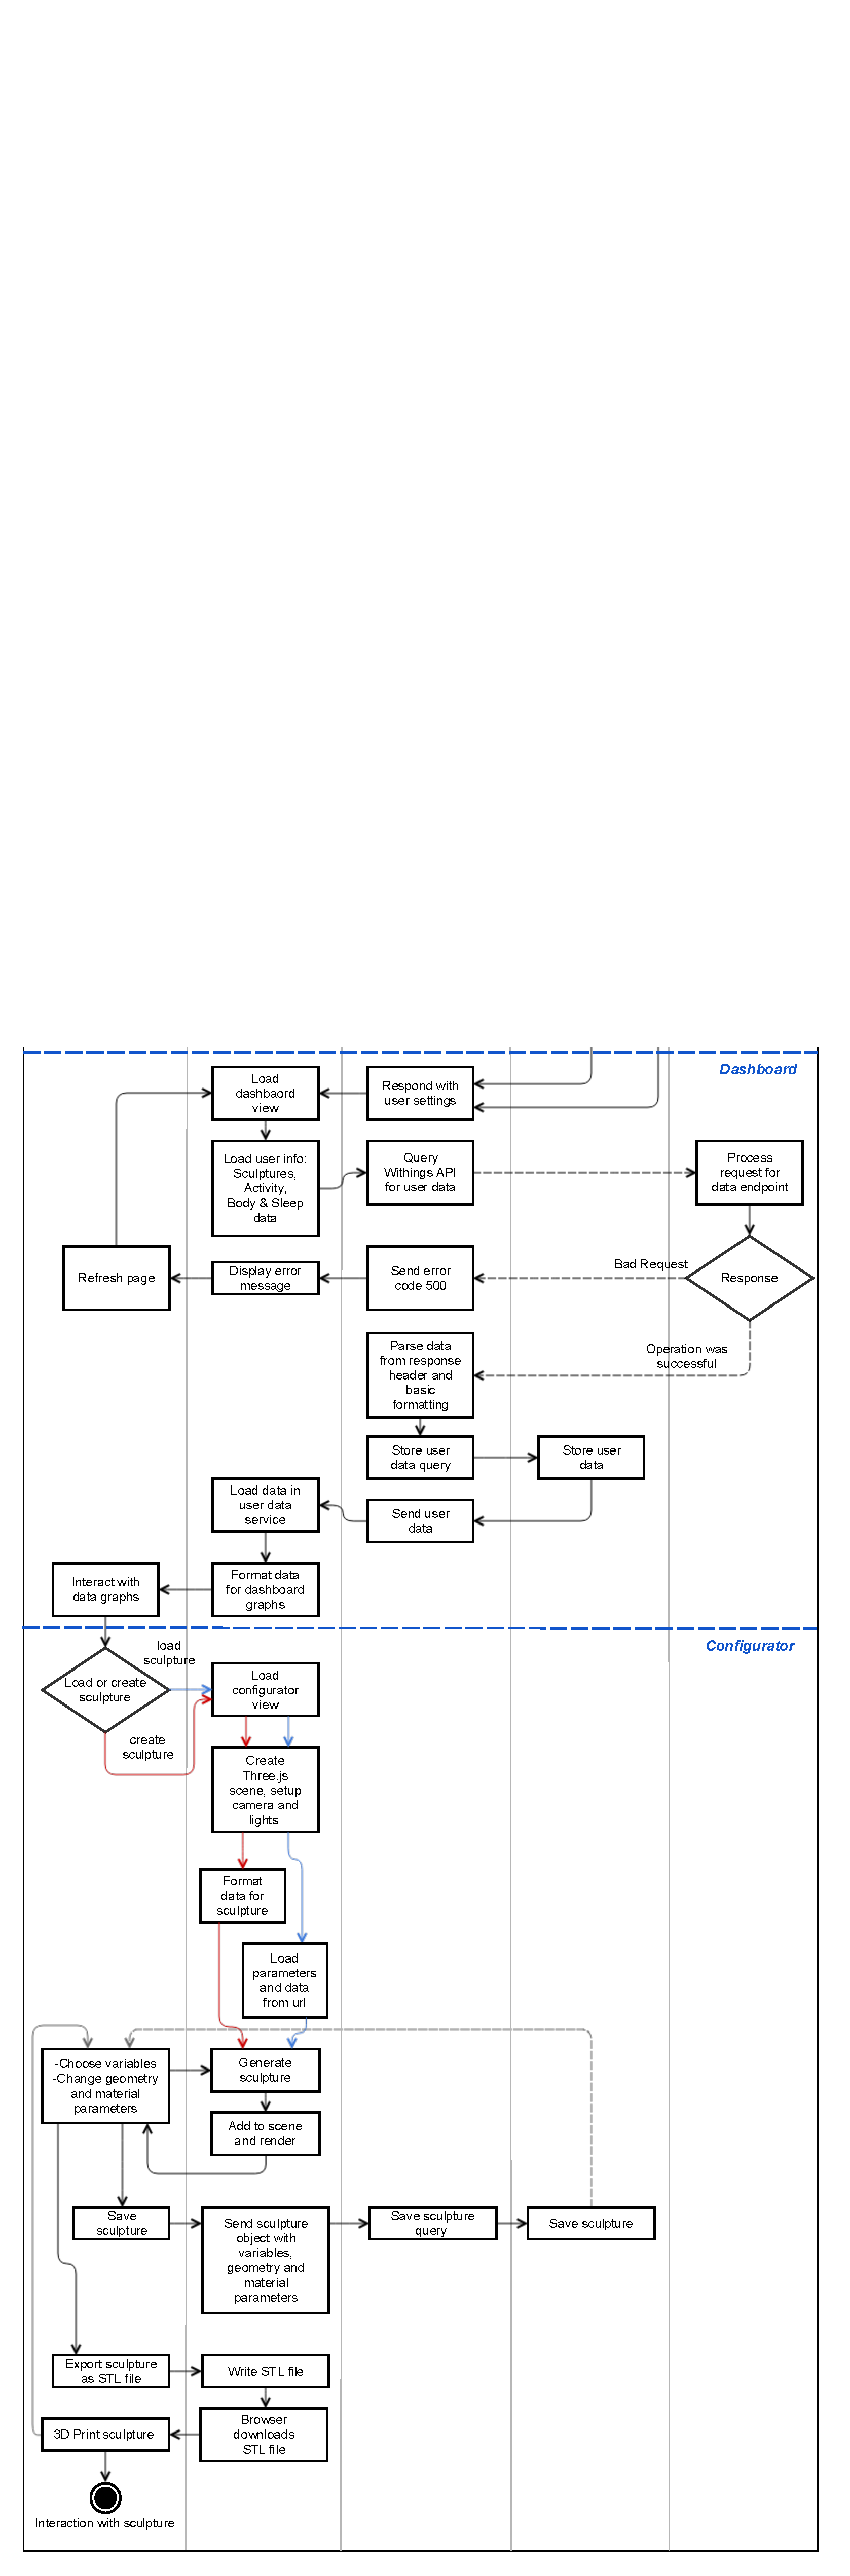
\includegraphics[width=0.86\textwidth]{Configurator/img/flowdiagram}
  \caption{Activity Sculpture web configurator's flow diagram part 2}
\label{fig:flowdiagram}
\end{center}
\end{figure}

\subsection{Configurator}
\subsubsection{Sculpture Generation \& Rendering}
Real time visualization
\textbf{WebGL} \textit{Threejs}\cite{cabello2010three}

\subsubsection{Sculpture Manipulation}

\label{sub:sculpturegeneration}
\subsection{Backend}
\subsubsection{Withings API Integration}
\label{sub:ApiIntegration}

Authentication 
\textbf{Passport}\cite{passport} 
\textbf{OAuth} \cite{hammer2010oauth}

Querying user data
\textbf{Withings-API}\cite{withingsApi} 
\textit{RESTful Web services} \cite{Fielding:2000:PDM:337180.337228}
\textbf{WebRTC}\cite{webrtc}
\textbf{SocketIO}\cite{socketio} 



\subsubsection{Data Processing}
\subsection{Challenges}
\end{document}
%______________________________________________________________________

\cleardoublepage
 % -*- root: ../medieninformatik-arbeit.tex -*-
\documentclass[../medieninformatik-arbeit.tex]{subfiles}
\begin{document}
\section{User Study}
\label{ch:study}
In order to test the implemented functionality and interaction concepts in the web configurator for guiding users in the visualization and customization process in an enjoyable yet efficient way, a user study was developed. The user study was comprised of a thinking aloud usability test with a small group of participants and an online test both including the same questionnaire. For ensuring the configurator was importing the data from the Withings API the author wore the fitness tracker every day for a time span of 2 months to generate enough data to work with. The specifics of the design of the user studies and the questionnaire as well as the obtained results will be discussed in the following sections. 

\subsection{Study Design}
The first part of the test for the usability of the web configurator was to perform a thinking aloud test. The thinking aloud protocol first introduced by Clayton Lewis in \cite{lewis1982using}, allows designers and developers to evaluate the usability of their system by letting a user speak out loud their thoughts as they use it. Users speak out of the content of their working memory which is driven by attention \cite{lewis1993task}. The basic concept of the thinking aloud protocol is to put users in front of a prototype of the system. Then developers have to chose a task for the user to solve in the prototype. Users are then filmed while they solve the task and speak their thoughts while using the prototype. Normally a thinking aloud usability test is performed with small number of participants raging from 5 to 10 participants, although some studies have been made that show that a usability test with 20 participants reveals up to 95\% of the problems in a system \cite{vande2008beyond}. 

For the purposes of this work the thinking aloud test was designed as follows. The users would sit in front of a laptop running the web configurator from the web server, meaning not the local development version was ever used but the live version available to the public. An informative text was designed (see appendix \ref{App:userstudy:consent}) that explained users the purpose of the web configurator, the task they were to perform and the concept of thinking aloud. This text also included a consent form for allowing the author to record a screen cast of their performance with an audio recording of their voice. The task to solve by users was to create a new sculpture, manipulate it to their contempt and save the sculpture when finished. After the sculpture was saved users were redirected to the questionnaire done in the Google Froms platform \cite{googleforms}. Due that it was not required for the participants to have their own Withings account, users started from the dashboard which gave them at the beginning an overview of the available data and also of the saved sculptures by other users. In this way it was possible to see if the designed process for creating a new sculpture was understandable for users. 

As discussed in the implementation chapter of this work, one of the requirements was to develop a working version and deploy it in a web server for the general public. So that anybody with a Withings account can log in and start visualizing their data. The purpose of this was to study how different data sets generate different sculptures. It was also of high interest for this work to receive feedback from the quantified self community, as the familiarity and interest for gaining insight from visualization of personal activity data is highly sought after in this community and activity sculptures are fairly new to the public. In order to achieve a high exposure of the web configurator in the quantified self community several platforms were chosen to present the web configurator. Although no exclusive forum for Withings users was found, a Withings user group was found in a sub page from the news aggregator website Reddit \cite{redditwithings}. The configurator was also introduced in the official quantified self forum \cite{qfselfforum}. Lastly the author contacted the organizers of the Munich quantified self meetup \cite{qfselfmeetup} for the possibility of introducing the web configurator in an upcoming meeting. Users that accessed the web configurator through the forum posts were first greeted with a consent dialog that explained the concepts of the project and stated it was only for research purposes related to this work. Only after users agreed with the terms of use they were able to login into the system. Also after saving a sculpture users were redirected to the questionnaire. 

To make the most out of online tester's participation, the use of an analytics tool was required. Analytics tools help web sites owners to gather information about what pages, for how long and from where users visit. Through the gathered information website owners can make changes to improve the visitors experience and translate this to higher revenues \cite{peterson2004web}. Another functionality web analytics offer is the tracking of mouse clicks which are used to generate event logs and in some cases even heat-map images that visually display what parts of the interface receive the most clicks. The web configurator makes use of the Inspectlet web analytics tool \cite{inspectlet} to track traffic and generate heat-map images of click events. Another nicety of the Inspectlet service is the ability to record videos of user sessions. This provides almonst the same results as the screen-cast recordings performed for the thinking aloud test. Other analytics tools were considered for this work like Hotjar \cite{hotjar} and Crazyegg \cite{inspectlet} all of which provide more or less the same functionality but with different price ranges. Inspectlet showed to be easily implementable through a short code snippet that is embedded to the index.html file of the web configurator. 

\subsection{Questionnaire}
The questionnaire was designed to gather qualitative data about the implemented web configurator and the designed activity sculpture. In total 35 questions were developed to question users about 3 main subjects: web configurators in general, the activity sculpture web configurator and the activity sculpture. The questionnaire was composed of questions that users could answer in some cases by selecting given options or in other cases through Likert scales that went from strongly agree to strongly disagree. It was important to ask users about any previous experience with web configurators in order to better estimate the familiarity of users with such systems. Users were also asked about their perception about the value added to any product by making it customizable and if they thought customizable products tend to be sold at higher prices. The familiarity of users with fitness trackers and physical activity habits was important to be able to have an idea of how active participants were. Regarding the implemented activity sculpture configurator users were asked about the attractiveness of the interface, ease of use and learnability. Feedback for the designed controllers was also wanted, therefore the questionnaire included some questions about the complexity of the controls, the understandability of label descriptions and visual feedback from updating the sculpture. User's opinion regarding the activity sculpture is equally important as it is the the product of the configurator and will influence the user's experience with the configurator. In this area users were asked about which visualization style they found most appealing, any attachment they felt to the generated sculpture, interestingness, the likeness of them using the configurator in a commercial context, willingness to expand the interaction of the sculpture to wearable objects, complexity of the sculpture, interest in more sculpture variations  and the feasibility of them sharing the sculpture with friends and relatives.
Finally users were asked about the overall experience of using the activity sculpture configurator and were offered a field for writing any comments or thoughts about the configurator. 

The developed questionnaire can be found in the appendix \ref{App:userstudy:questionnaire}.

\subsection{Participants \& Procedure}
In a time span of 3 days participants were selected randomly by asking students in a university building to participate in the thinking aloud test, resulting in 5 participants gathered. For the thinking aloud test a table in a quiet area was set up with the laptop, the instructional text and the consent forms. After reading and signing the consent, the recording of the screencast with audio was started  users started to use the configurator speaking their thoughts out loud. After the sculpture was saved the recording was stopped and users continued to answer the questionnaire. 

For the quantified self forum and the Withings Reddit subgroup one post was written in each platform and for a period of one month, traffic from this website was tracked and screencasts were recorded with the Inspectelt service. 

\subsection{Results}
Between the thinking aloud and the online testers 9 survey answers were gathered. Participants had an average age of 25 ranging from 19 to 35. 6 of them were males and 3 females. The post about the web configurator in the Reddit Withings user group had 45 views  and in the Quantified self forum 174 views summing up a total of 219 viewers in the test month. The  Inspectlect analytics service recorded 55 sessions, because of the free version used for this work which was limited to 4 recordings per day. From these 55 recordings Inspectlet showed that the visitors came from distinct parts around the globe including China, France, the U.S., Mexico, Canada, Switzerland, United Kingdom and Denmark. Unfortunately the analytics show that the duration of the visits were as long as a couple of seconds. Causes of this user behavior can be the consent window that is displayed at the beginning. Maybe visitors get discouraged by the warnings regarding data privacy and because the website does not show them any information that motivates them to stay users leave. Another problem encountered was an authentication bug in the application that after granting permission to the configurator to access their resources from the Withings server, redirected users to ``Bad Gateway'' or ``500 Internal Server Error'' messages making it impossible for visitors to use the configurator. This was noted by a visitor from the Reddit post and it might have scared visitors off. Until the bug was fixed some weeks had already passed by and instead the author asked directly to friends to use the configurator with his own credentials. Added to this errors, it was not possible to present the configurator in the Munich Quantified self meetup due to organizers not having enough speakers for the evening. Unfortunately the online testing phase was a failure and the goals of evaluating sculptures generated with different data and gathering feedback from the quantified self community were not achieved. 

From the participants that did answer the questionnaire the following results were gathered. Participants responded to have very low experience with web configurators or 3D software that also require them to navigate objects in 3D space with only one participant that had used a web configurator before and two participants that had intermediate to no experience with 3D software. The user that had experience with web configurators described his experience as neutral. Even though only one participant from the group had used a web configurator, everybody assured that customizable products seem more attractive to them and 66\% felt customizable products tend to be more expensive. Although web configurators seem to be not as widespread for this user sample, customization of product is perceived as an added value to the product and is attractive to customers. 
Regarding their activity habits almost half of participants does not have any exercise habits and one third exercise few times a week, leaving the rest to only sporadic work out session. The usage of tracking devices was only adopted by one user and stated to use fitness trackers under the other category. The same user confirmed he had experienced a motivation boost from using it. Nonetheless, the rest of the users but one, had considered starting using a fitness tracker. Participants opinion regarding fitness trackers usage seems to be highly influenced by their activity habits as most participants are not very active, but nonetheless fitness trackers seem interesting to most of them. 
Over half of the participants found the sculpture to be aesthetically appealing and 71.4\% found the normal visualization style to be the most attractive. The greater half of participants felt neutrally attached to the sculpture with the rest of participants leaning toward stronger attachment. Overall participants found it interesting to see their data visualized in a sculpture with 60\% answering positively. The survey showed participants were unsure if they would use the configurator regularly to visualize their data as one half was leaning more towards using it and the other half against it. Participants showed to be neutrally interested in the possibility of paying to get their sculpture 3D printed but half of them were willing to wear their sculpture as an accessory. Sharing the sculpture with friends and relatives was perceived as positive and most users answered positively. Towards the need of a more accurate visualization of the data in the sculpture, users appeared to be rather neutral. Two thirds of participants were rather satisfied with their sculpture and one third was neutral about it. 
The greater half of users expressed they found the configurator's user interface to be aesthetically appealing and also easy to use. The system was graded to be easy to learn by 77\% of participants. 70\% of users answered the labels describing the UI controls were helpful and the transformations controls performed on the sculpture were also understood by 80\% of participants. Participants found the available configuration options to be enough and 90\% of participants described the sculpture updating instantly after changing controls to be very helpful. The dashboard and the sculpture gallery were regarded as helpful to get a summary of the gathered data and of the collected sculptures over time. Two thirds of participants answered they would have liked to have more sculpture designs to choose from.
Finally 80\% of users expressed they thought the configurator's functionality was useful and all of them said they would use it again. As final thought only one person expressed the variables showed in the activity chart to be somewhat confusing because activity and calories burned were combined in the same chart. The questionnaire results are also available in appendix \ref{App:survey:results}.

The thinking aloud usability test was performed successfully with only some minor technical difficulties with Google Forms which crashed once making it impossible for one participant to answer the questionnaire. The video material gathered from the thinking aloud tests was evaluated with the goal of finding errors in the user interface and also to understand the thought process of users while utilizing the configurator. For this a spreadsheet was developed containing 4 fields for features missed by the user, UI widget problems, user comments and remarks from the author. In general users performed fairly well and experimented with most features of the configurator. The widgets that were missed by users were the labels toggle missed by 4 users, the wireframe toggle missed by 2 users and only one user missed the geometry tab for the left control panel. Furthermore 2 users had difficulty operating the toggle button. It is important to mention that the toggle button implemented in the configurator with the Angular-material framework resembles the toggle button found in most smartphones nowadays which is primarily designed for touch gesture based interaction. Due that the configurator was designed as a desktop application the interaction with this kind of toggle button is not suitable for mouse operation. Users tried to wipe the button with the mouse which did not activate the toggle. Instead users should have just clicked the toggle to make it change its value. It was interesting to see how users were discovering the concepts behind the activity sculpture and the overall functionality of the configurator. The positioning of the new sculpture button in the dashboard was easy for users to find and was described as an``obvious'' way to create the new sculpture. Two users commented it was difficult for them understanding what the interpolated mode did to the sculpture. The purpose of the sculpture was questioned by two users, one of them stating that data visualization should be precise. The same user was expressed to be irritated by the normalization of the data and described it as illogical. Users also made comments when they discovered that the data in the sculpture is visualized overt time and axes can be added to the sculpture. One user was surprised to see how much data is possible to gather about one's activity and also commented it was difficult to note any difference in the sculpture when adding many variables. On the author's remarks, users sooner or later intuitively navigated the sculpture by clicking and dragging even though there are no instructions in the configurator. In general users did not make any comments about the dashboard an started the process of creating a new sculpture right away. The ``SPO2'' label was also new to most users as many of them asked its meaning. Interestingly one user did not understand that he was able to add variables to the sculpture by clicking on the buttons and asked where could he enter new data. An interesting observation of self reflection was made by a user while navigating the sculpture stating ``this day I made a lot of intense activity'' showing how even though it was not their data, participants tried to see the sculpture as their own. 

Because for the online test and for the thinking aloud test the deployed configurator in the public server was used, all participant's click events were also tracked by the Inspectlet analytics tools. Inspectlet generates three different heatmap images: click events, eye-tracking and scroll heatmaps. The eye-tracking heatmap is not generated through the use of tracking cameras but is an approximation based on mouse movements and clicks. Scroll heatmaps allow web site owners to see until which point users scroll through the page. For the purposes of this work only the click heatmap was used (see figure \ref{fig:heatmap} and appendix \ref{App:survey:heatmap:click}). The generated heatmap shows through the bigger marks how users clicked mostly on the left control panel. Unfortunately its not possible to see if users were selecting variables or operating controls in the top area. Nonetheless the heatmap shows users experimented with different variables and controls heavily. In the middle section many marks are also visible from navigating the model in 3D space, enforcing the intuitiveness users have to manipulate the sculpture in 3D. Because of the bigger mark on top of the data tab it seems that users experimented more with adding variables than with geometry parameters. On the right side it seems users did not experiment a lot with the color picker as it remained fairly clean of marks. The export tab seems to have been selected frequently as it presents heat marks.

\begin{figure}[h]
\captionsetup{width=\textwidth}
\begin{center}
  \includegraphics[width=0.7\textwidth]{Appendix/questionnaire/click_heatmap}
  \caption{Inspelect analytics generated click heatmap}
\label{fig:heatmap}
\end{center}
\end{figure}

To summarize the results, it seems web configurators are not as common as thought, but users are willing to experiment and the customization of products remains interesting for most users. The web configurator performed very well as users found it to be ease to operate and also easy to learn. Other than the toggle button all controls performed well and the labels were also understood by users. Interestingly users spend more time experimenting with different combinations of variables mapped to the sculpture than customizing the geometry. The activity sculpture was also perceived as aesthetically appealing and users seem to have a neutral opinion towards the level of abstraction used in the sculpture. The interpolated visual style seems to be somewhat confusing to users as they did not understood well what was happening in the sculpture. It seems the usefulness of activity sculptures is not entirely understood as it was questioned by some users. Even though the online test on the forums and the meetup failed, the usability test and the few online tests still produced helpful insight. 

\subsection{Limitations}
Among the limitations of the user study was the short available time left due to the prolonged development phase. Initially the goal was to perform several smaller user studies but again the development required more time than expected and the user studies had to be shortened to a usability test and an online test which unfortunately failed. 

Limiting the configurator to work only with the Withings API had its advantages and disadvantages. It provided users a very simple form of importing their data but the Withings user base seems to not have a dedicated forum and the sense of community for sharing experiences between users is not present. As in the research phase for the best fitness tracker to work with these aspects were not entirely considered the user study suffered. A solution for this would have been to contact at least a small group of Withings or other brand users and perform a more in depth study with them. By attending the Munich Quantified self meetup the author expected to reach more Withings users and get more feedback from more advanced quantified self practitioners. Sadly the inactivity of the community in Munich did not facilitated a meeting in the time frame of the development of this work. 

The login bug that impeded users to access the web page affected the success of the online study greatly. The difficult part of fixing the bug was its reproducibility. The Withings authentication requires the URL address starting the \textit{OAuth} flow had to be the same as in the callback URL address. The posted URL in the forums contained ``www.'' at the beginning and in the callback the URL not which translated in the redirect to ``bad gateway'' issue. Unfortunately the bug took one week to fix in between performing the user study. Another factor for the failure of the online test seems to be the consent message displayed at the beginning. Admittedly not many options were considered for displaying the consent message. In this place it would have been helpful to give visitors a friendlier welcome site, showcasing some attractive aspects of the project inviting users to log in and try out the configurator. 

The conclusion of this work and the possible improvements to the configurator will be discussed in the following chapters respectively. 

\end{document}

%______________________________________________________________________

\cleardoublepage
\chapter{Conclusion}
\label{ch:conclusion}
\section{Conclusion}

%______________________________________________________________________

\cleardoublepage
\label{ch:future}
\section{Future Work}

%______________________________________________________________________
%Abbildungsverzeichnis erzeugen - normalerweise nicht n�tig
\cleardoublepage
$%\pagestyle{plain}
\listoffigures

%______________________________________________________________________
\cleardoublepage
\bibliographystyle{abbrv}
\bibliography{ma-thesis}

%______________________________________________________________________
\cleardoublepage
\appendix
\addcontentsline{toc}{section}{Appendix}
\section*{Appendix}
\section{Online Questionnaire} \label{App:questions}
\section{User Study Results} \label{App:results}
\subsection{Questionnaire Results} \label{App:results-questions}
\subsection{Heat Map Images} \label{App:results-heatimgs}
\section{Prototype Sketches} \label{App:prototypes} 
\subsection{Sculpture Prototypes} \label{App:proto-sculptures}
\subsection{Web Configurator Prototypes} \label{App:proto-config}

%______________________________________________________________________
\cleardoublepage
\fancyhead[LE,RO,LO,RE]{} % Keine Kopfzeile mehr oben auf jeder Seite
\cleardoublepage
\pagestyle{plain}
\addcontentsline{toc}{section}{Contents of the enclosed CD}
\section*{Contents of the enclosed CD}
\paragraph{Thesis}
\begin{itemize}
  \item \LaTeX\ Document   
  \item PDF File 
\end{itemize}

\paragraph{Presentations}
\begin{itemize}
  \item Initial presentation
  \item Final presentation
\end{itemize}

\paragraph{Activity Sculpture Web Configurator}
\begin{itemize}
  \item Prototype sketches  
  \item Source code
  \item Gitlab and Github mirrors  
  \item Instructions for deployment  
  \item Login Data
   
\end{itemize}    

\paragraph{Sculptures}
\begin{itemize}
  \item Prototype sketches 
  \item.stl 3D print ready example files 
\end{itemize}

\paragraph{User Study}
\begin{itemize}
    \item Questionnaire 
    \item Results
    \item Heat map images
  \end{itemize}      

\end{document}
